% ============================================================================================
\section{I2: Browser Visualizations in D3.js (Owner: Parthsarati Samanta, BT2024083)}
\label{sec:i2}
Both views are plain HTML/CSS/JavaScript with D3 v7.9.0~\cite{bostock2011} vendored locally, so there is no build step
(\fpath{infovis/i2_web/}, served with \texttt{python -m http.server}). Screenshots are produced by
\fpath{screenshots.py}. It drives Chromium through Playwright~\cite{playwright} at $1600\times900$ CSS pixels with device
scale factor 2, calling the same functions the UI controls call, so every screenshot state can be reproduced exactly.

\subsection{I2a: Parallel coordinates with edge bundling}
\textbf{Design.} There are eight axes~\cite{inselberg1985}, each with a scale suited to its data: linear for date, hour,
title length and upvote ratio; logarithmic for score ($\ge$1,115); symmetric-log for comments and crossposts, which contain
zeros; and a point (ordinal) scale for post type. The 2,000 records are those of Sec.~\ref{sec:derive}.

\textbf{Edge bundling.} We follow the cluster-based bundling idea for parallel coordinates~\cite{zhou2008,heinrich2013},
in the spirit of Holten's bundling strength $\beta$~\cite{holten2006}. For each group $g$ (k-means cluster, topic or post
type) we compute the centroid $\bar y_g^{(a)}$ of every axis $a$ in \emph{pixel space}, so log and ordinal axes are handled
uniformly. Between adjacent axes $a$ and $b$, each polyline gets two control points at $t\in\{0.25, 0.75\}$ of the gap:
\begin{equation}
y_t=(1-\beta)\,[\,y^{(a)}+t\,(y^{(b)}-y^{(a)})\,]+\beta\,[\,\bar y_g^{(a)}+t\,(\bar y_g^{(b)}-\bar y_g^{(a)})\,].
\end{equation}
The path is a monotone cubic (\texttt{d3.curveMonotoneX}) through the axis values and the control points. $\beta=0$ gives
plain polylines; $\beta\rightarrow1$ pulls every line between the axes onto its group's centroid line, while the line still
meets the axes at the record's true values (Algorithm~\ref{alg:bundle}). A slider changes $\beta$ live, and an option draws the
group centroid lines (dashed).

\begin{algorithm}[!t]
\caption{Cluster-centroid edge bundling for parallel coordinates}
\label{alg:bundle}
\begin{algorithmic}[1]
\REQUIRE records $R$, axis order $(a_1..a_m)$, scales $y_a$, group $g(r)$, strength $\beta$
\FORALL{groups $g$, axes $a$} \STATE $\bar y_g^{(a)}\leftarrow\mathrm{mean}_{r: g(r)=g}\; y_a(r_a)$ \ENDFOR
\FORALL{$r\in R$}
  \STATE $P\leftarrow[\,]$
  \FOR{$i=1$ \TO $m$}
    \STATE append $(x_{a_i}, y_{a_i}(r))$ to $P$
    \IF{$i<m$}
      \FORALL{$t\in\{0.25,0.75\}$}
        \STATE $s\leftarrow y_{a_i}(r)+t\,(y_{a_{i+1}}(r)-y_{a_i}(r))$; \ $c\leftarrow \bar y_{g(r)}^{(a_i)}+t\,(\bar y_{g(r)}^{(a_{i+1})}-\bar y_{g(r)}^{(a_i)})$
        \STATE append $(x_{a_i}+t\,(x_{a_{i+1}}-x_{a_i}),\ (1-\beta)s+\beta c)$ to $P$
      \ENDFOR
    \ENDIF
  \ENDFOR
  \STATE draw monotone-cubic path through $P$
\ENDFOR
\end{algorithmic}
\end{algorithm}

\textbf{Interactions.}
\begin{itemize}
\item \emph{Brushing} on every axis with \texttt{d3.brushY}. Several brushes combine with AND; selected lines keep the group
  colour and are raised, the rest fade to grey.
\item \emph{Drag-to-reorder}: dragging an axis title moves the axis, and lines are redrawn on the fly.
\item Colour/bundle grouping selector, hover tooltip with the post title and all values, a Reset button, a live count of
  selected records, per-group selected/total counts in the legend, and a text summary of the active brushes.
\end{itemize}

\begin{figure*}[!t]
\centering
\subfloat[Unbundled ($\beta=0$), k-means colour]{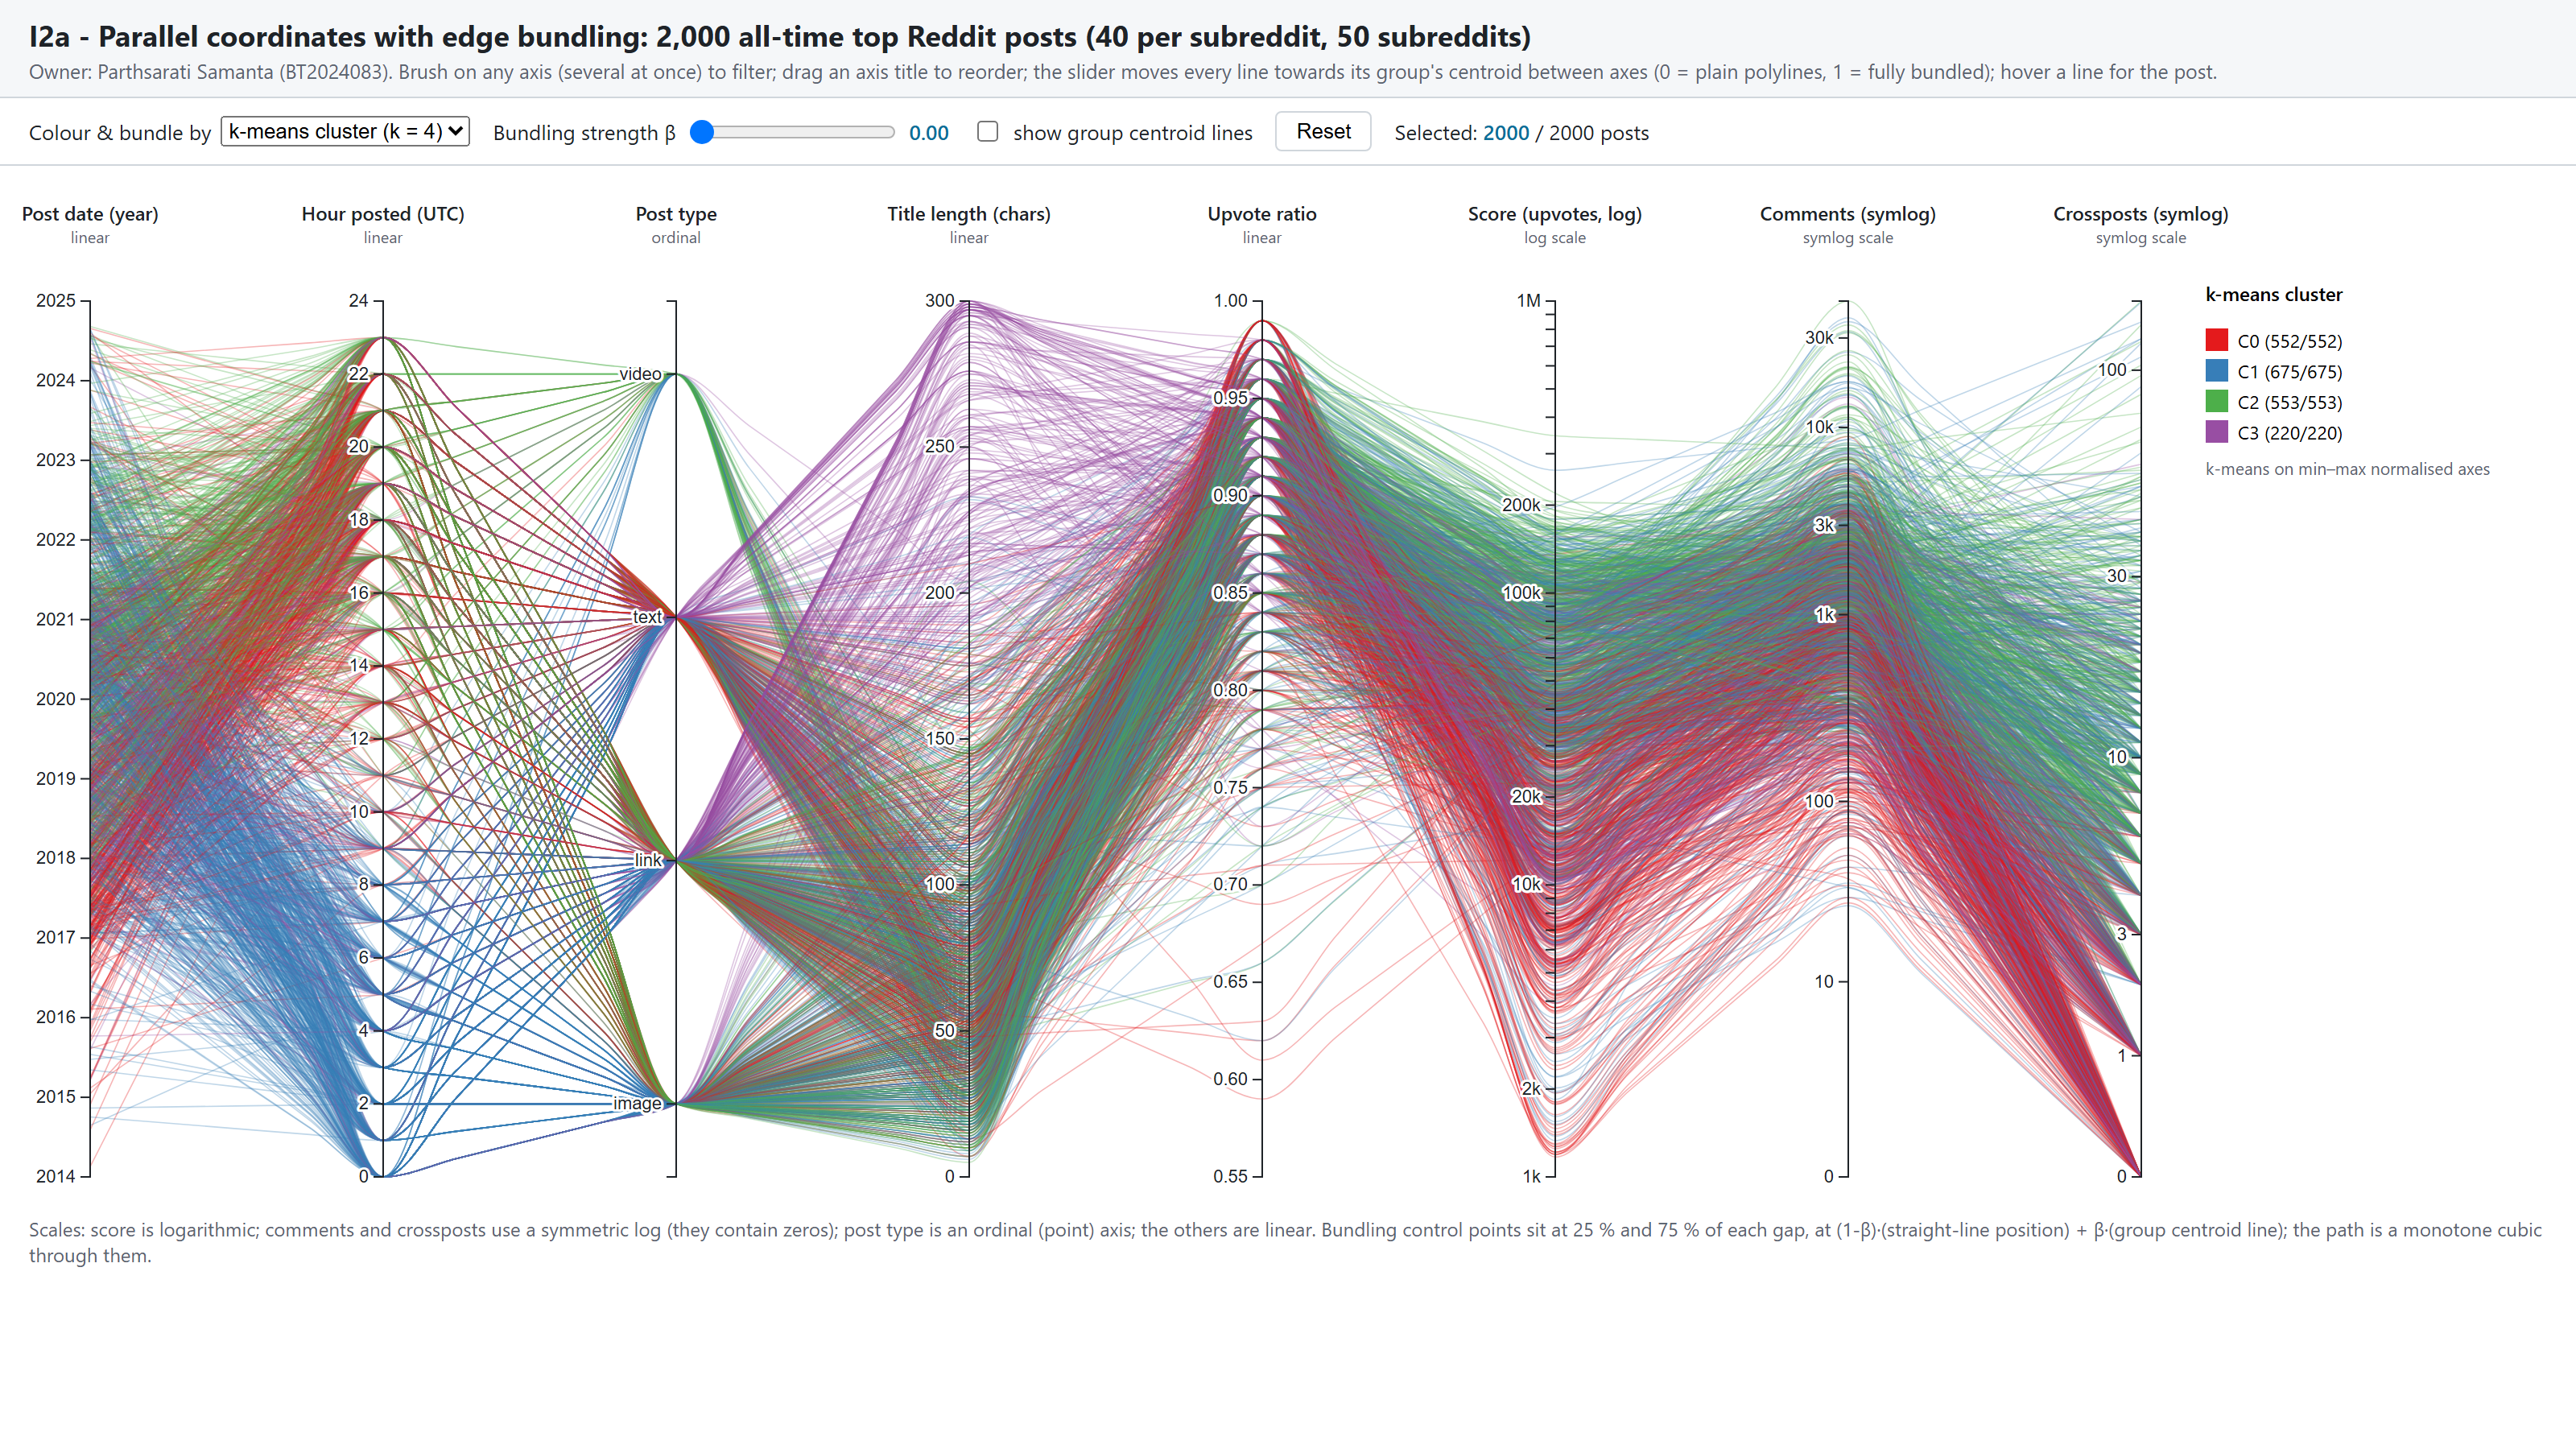
\includegraphics[width=0.495\textwidth]{Fig_31a_parcoords_unbundled.png}}\hfill
\subfloat[Bundled ($\beta=0.85$), k-means colour]{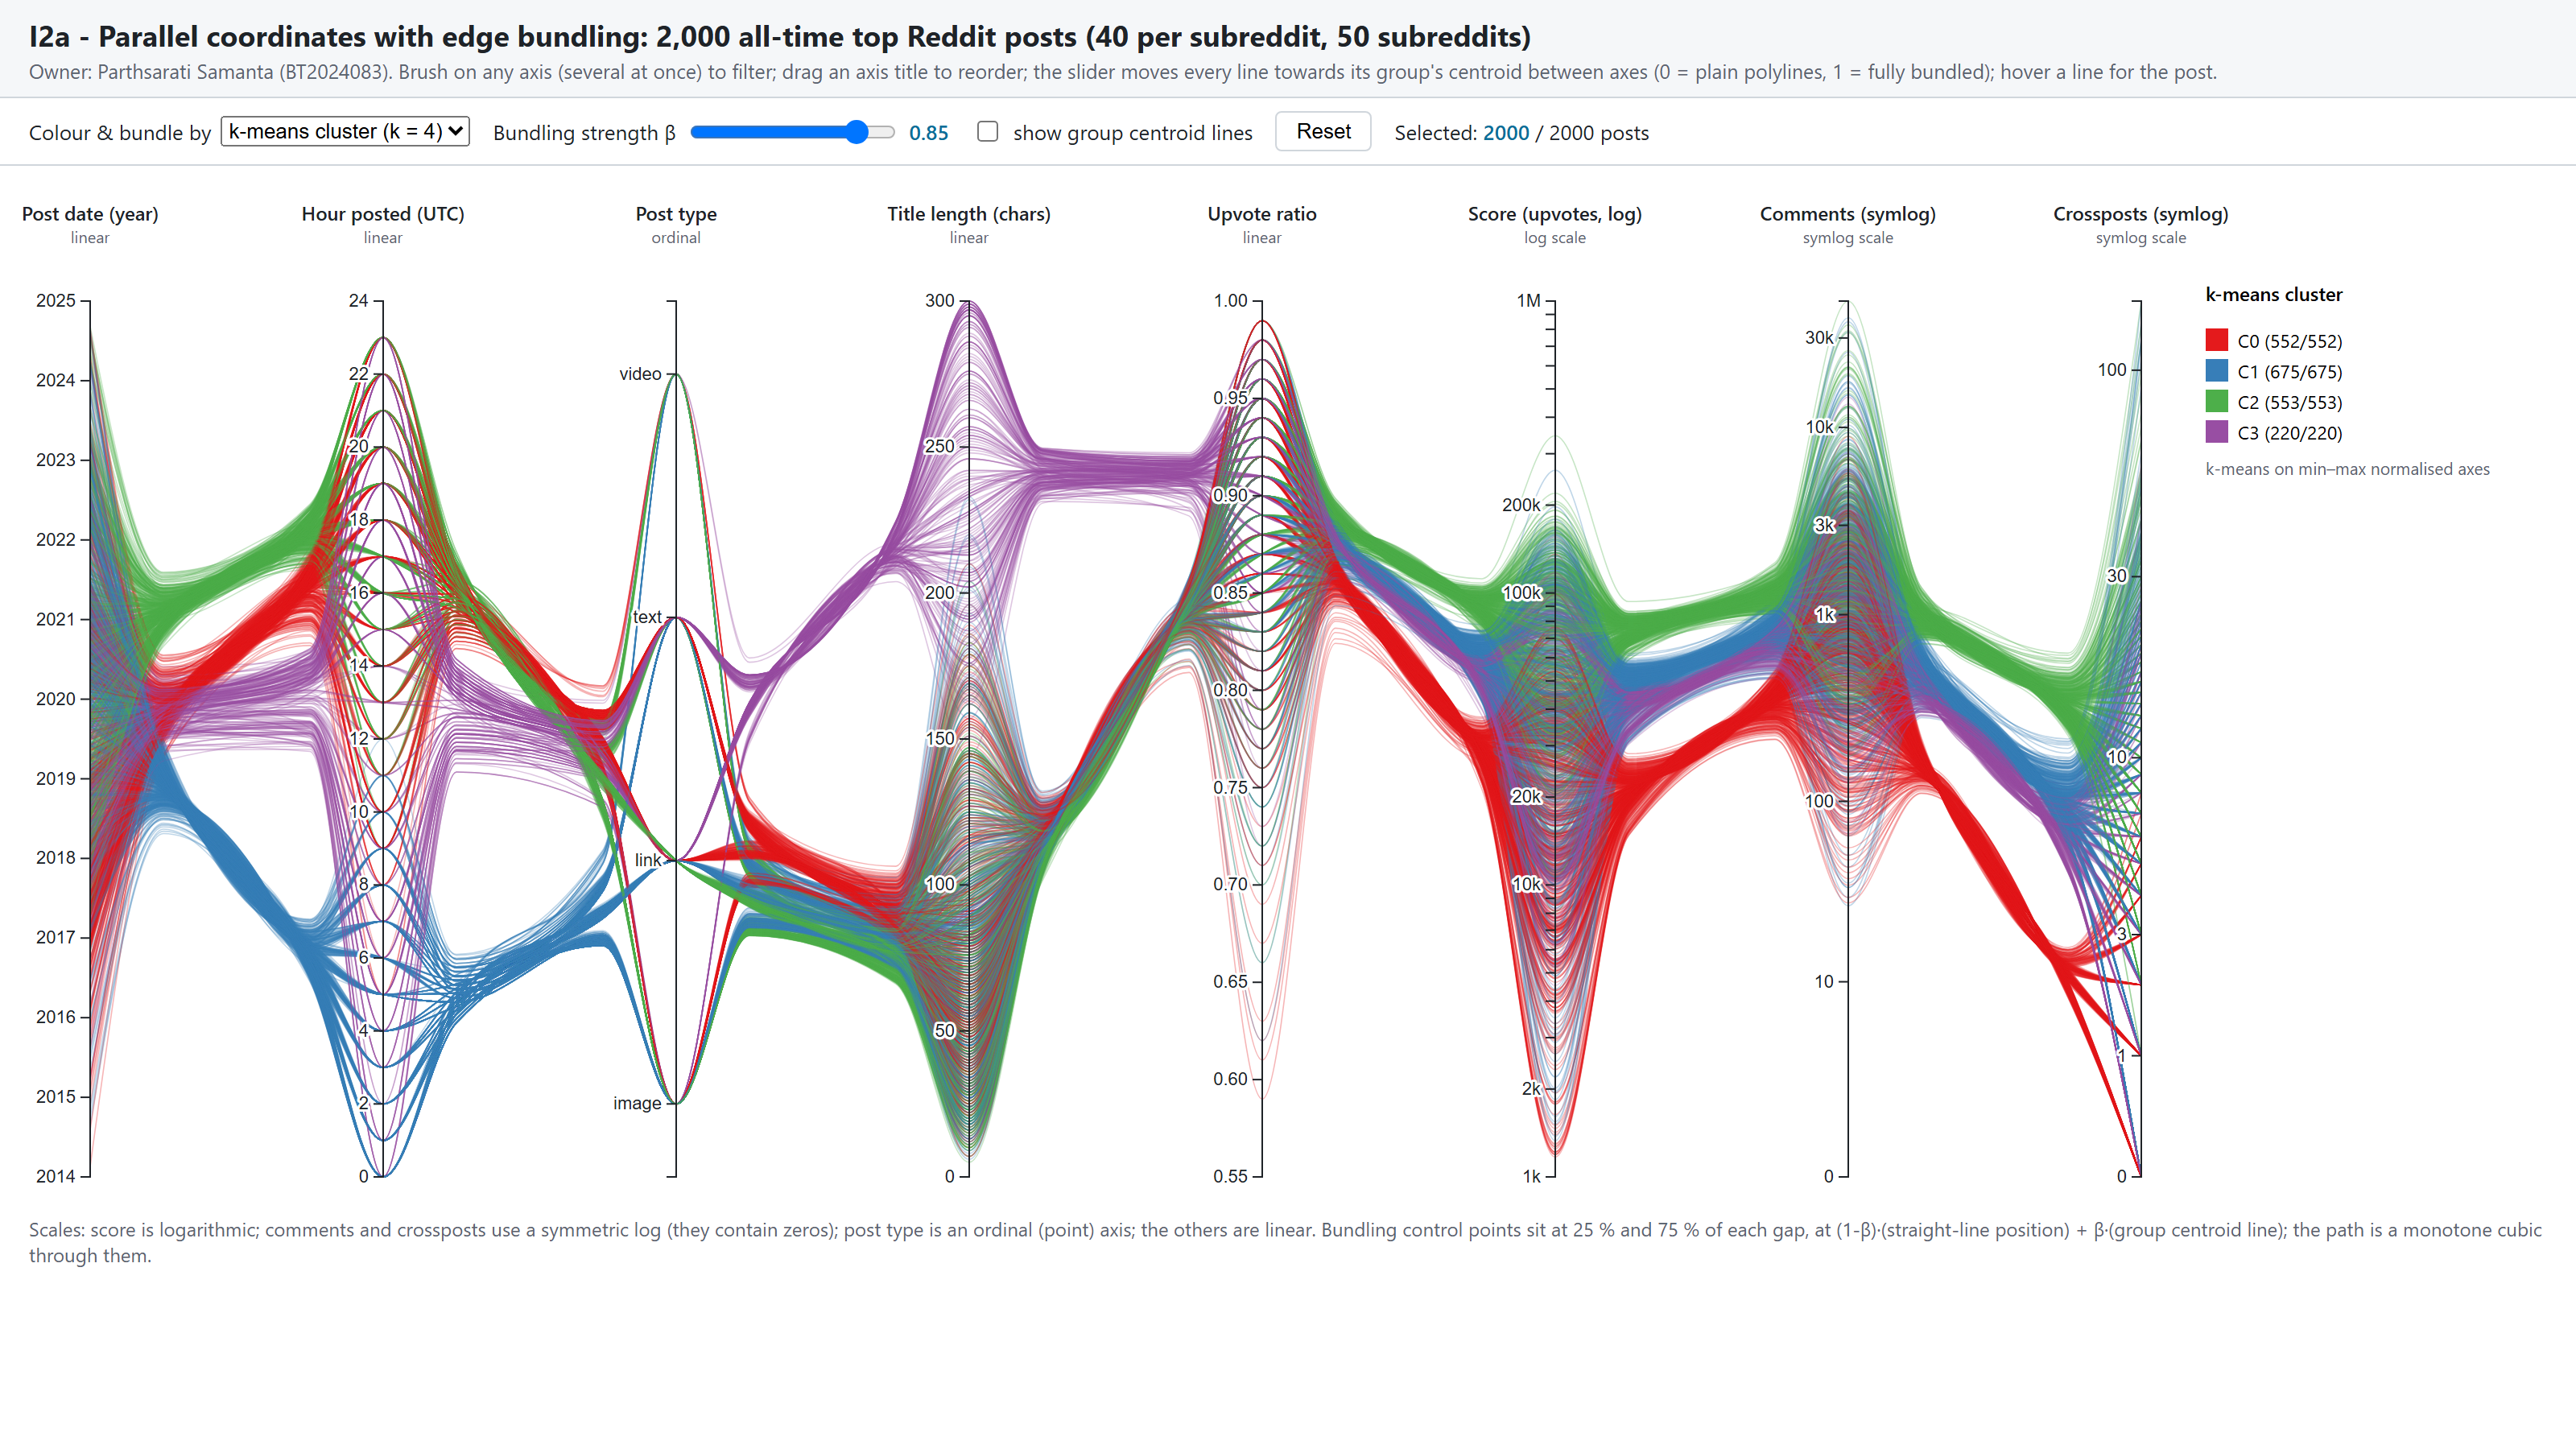
\includegraphics[width=0.495\textwidth]{Fig_31b_parcoords_bundled_kmeans.png}}\\
\subfloat[Bundled ($\beta=0.85$) by topic, with dashed centroid lines]{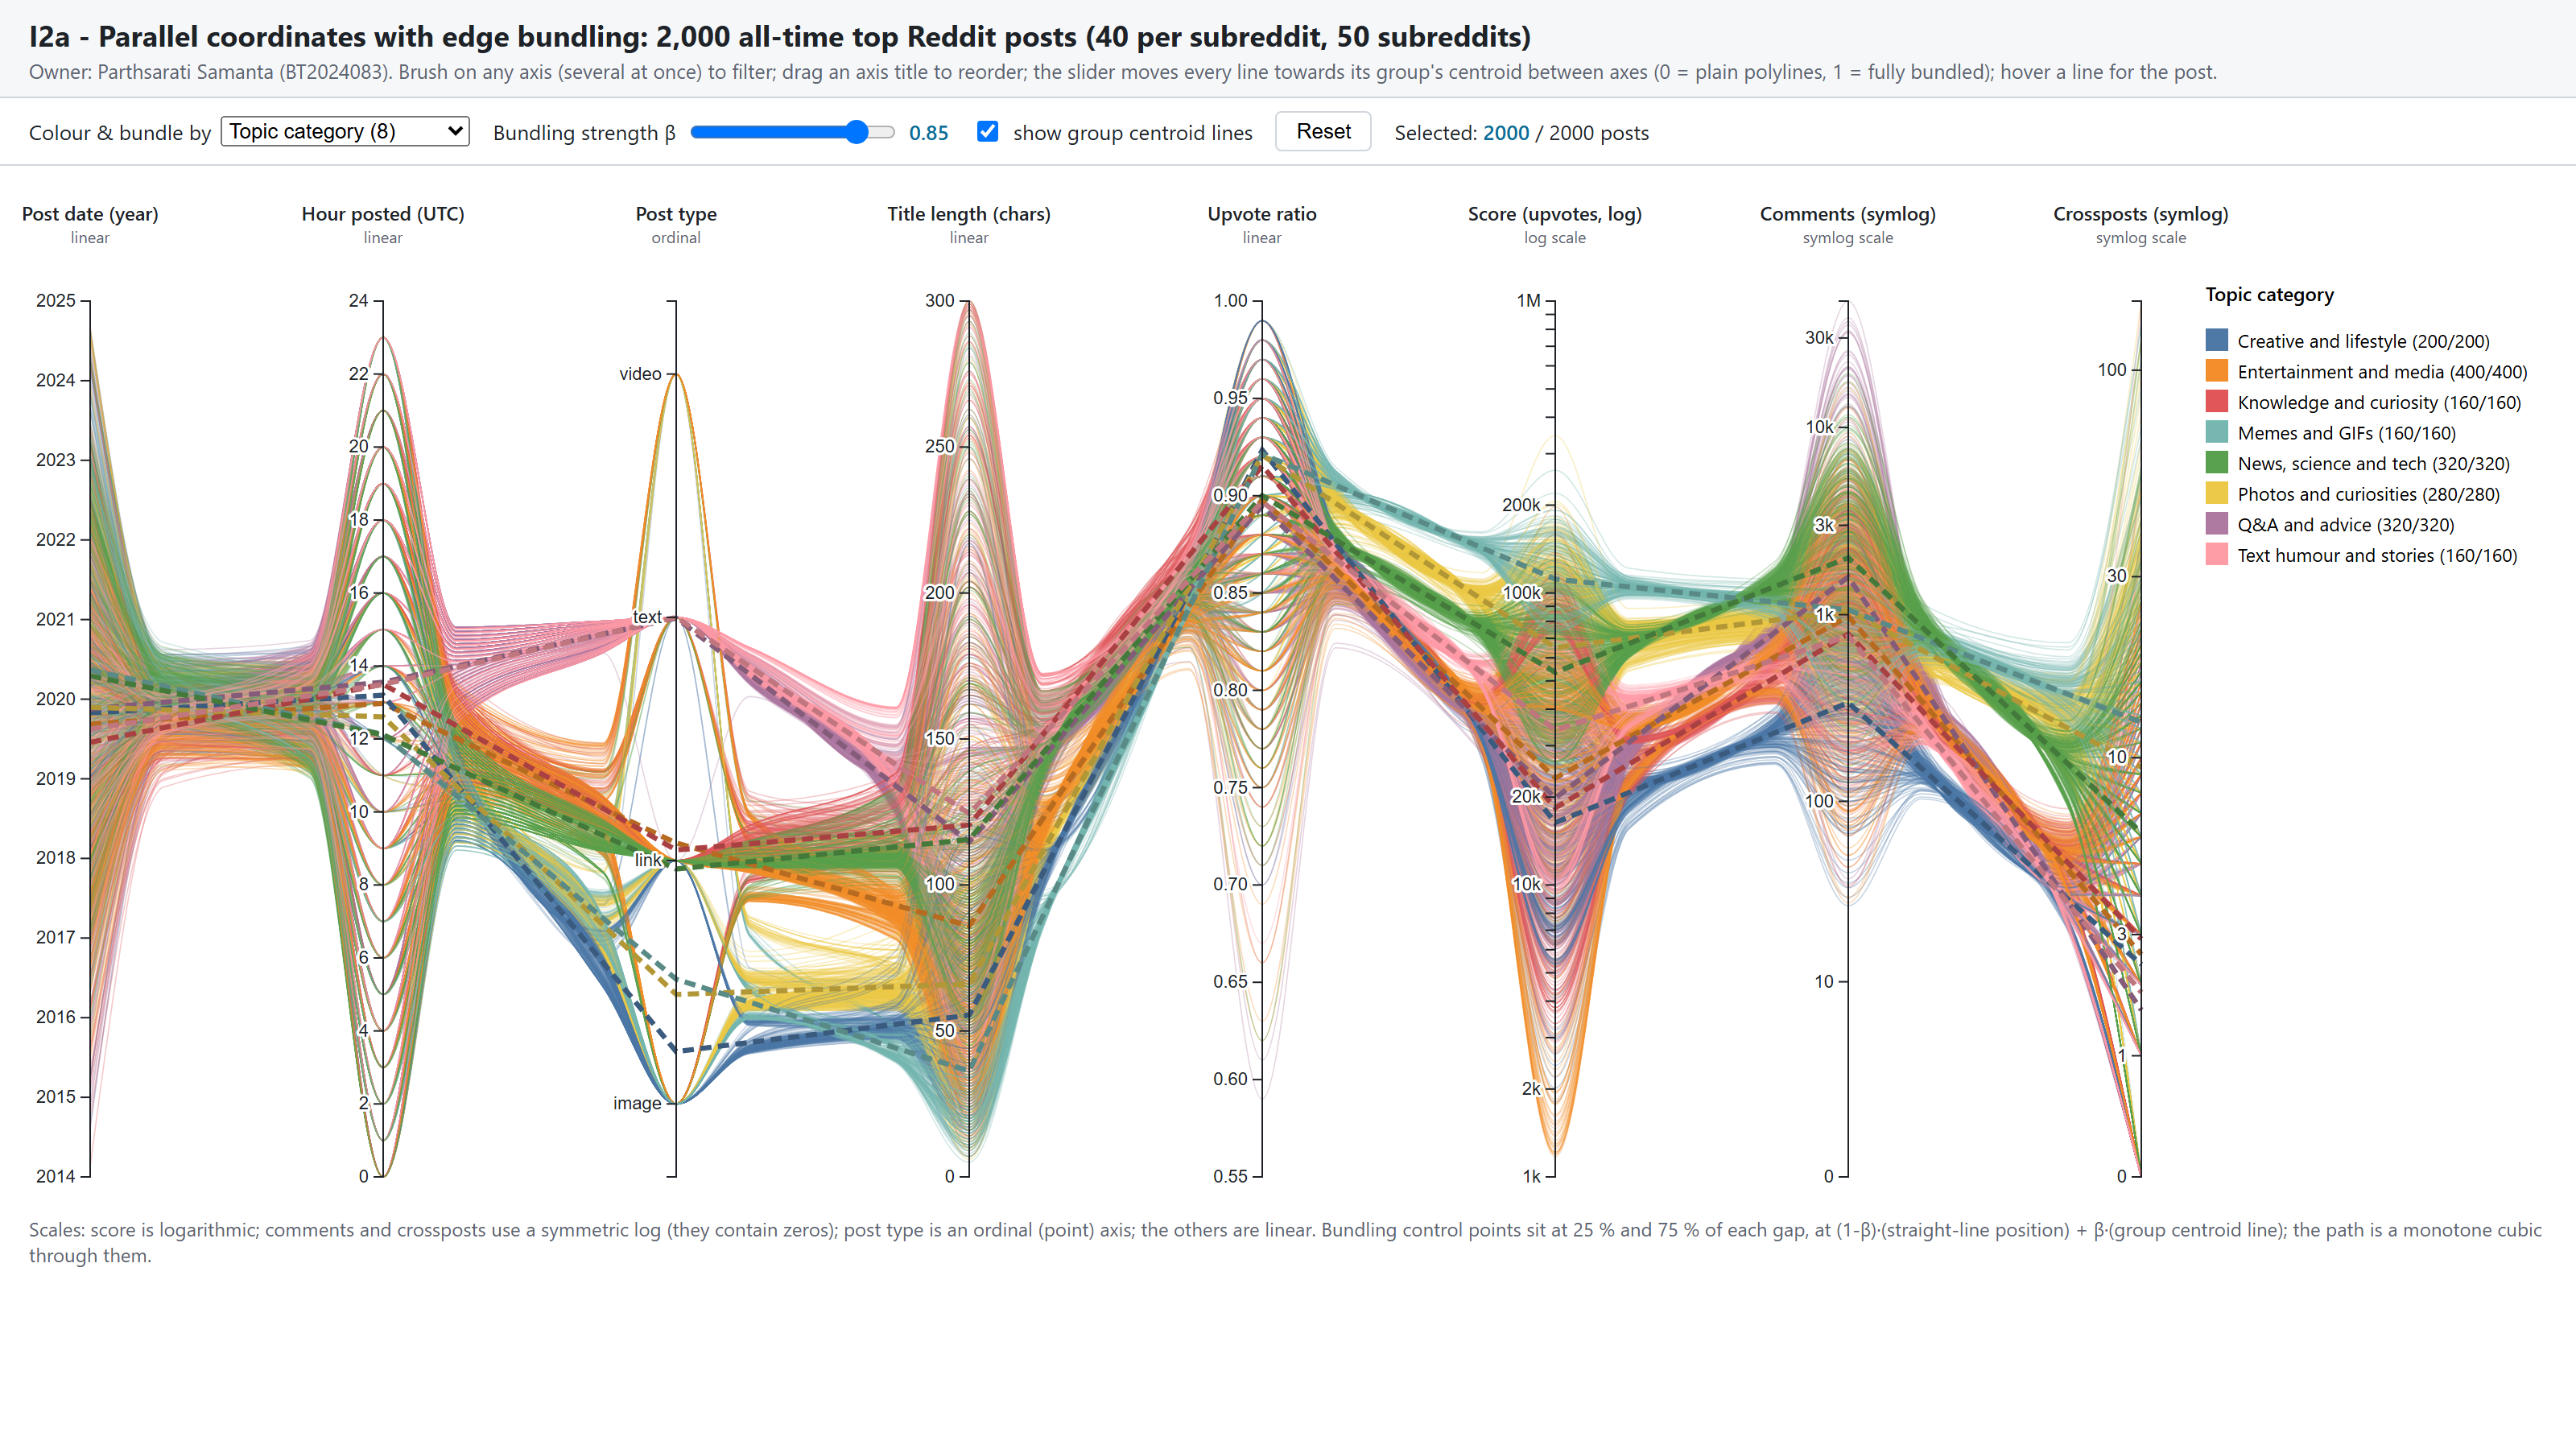
\includegraphics[width=0.495\textwidth]{Fig_31c_parcoords_bundled_topic.png}}
\caption{Parallel coordinates of 2,000 top posts: effect of edge bundling (I2a). Files \fpath{Fig_31a/b/c_*.png}.}
\label{fig:31}
\end{figure*}

\begin{figure*}[!t]
\centering
\subfloat[Brushes: score $\ge$60k AND post type = text; colour = post type]{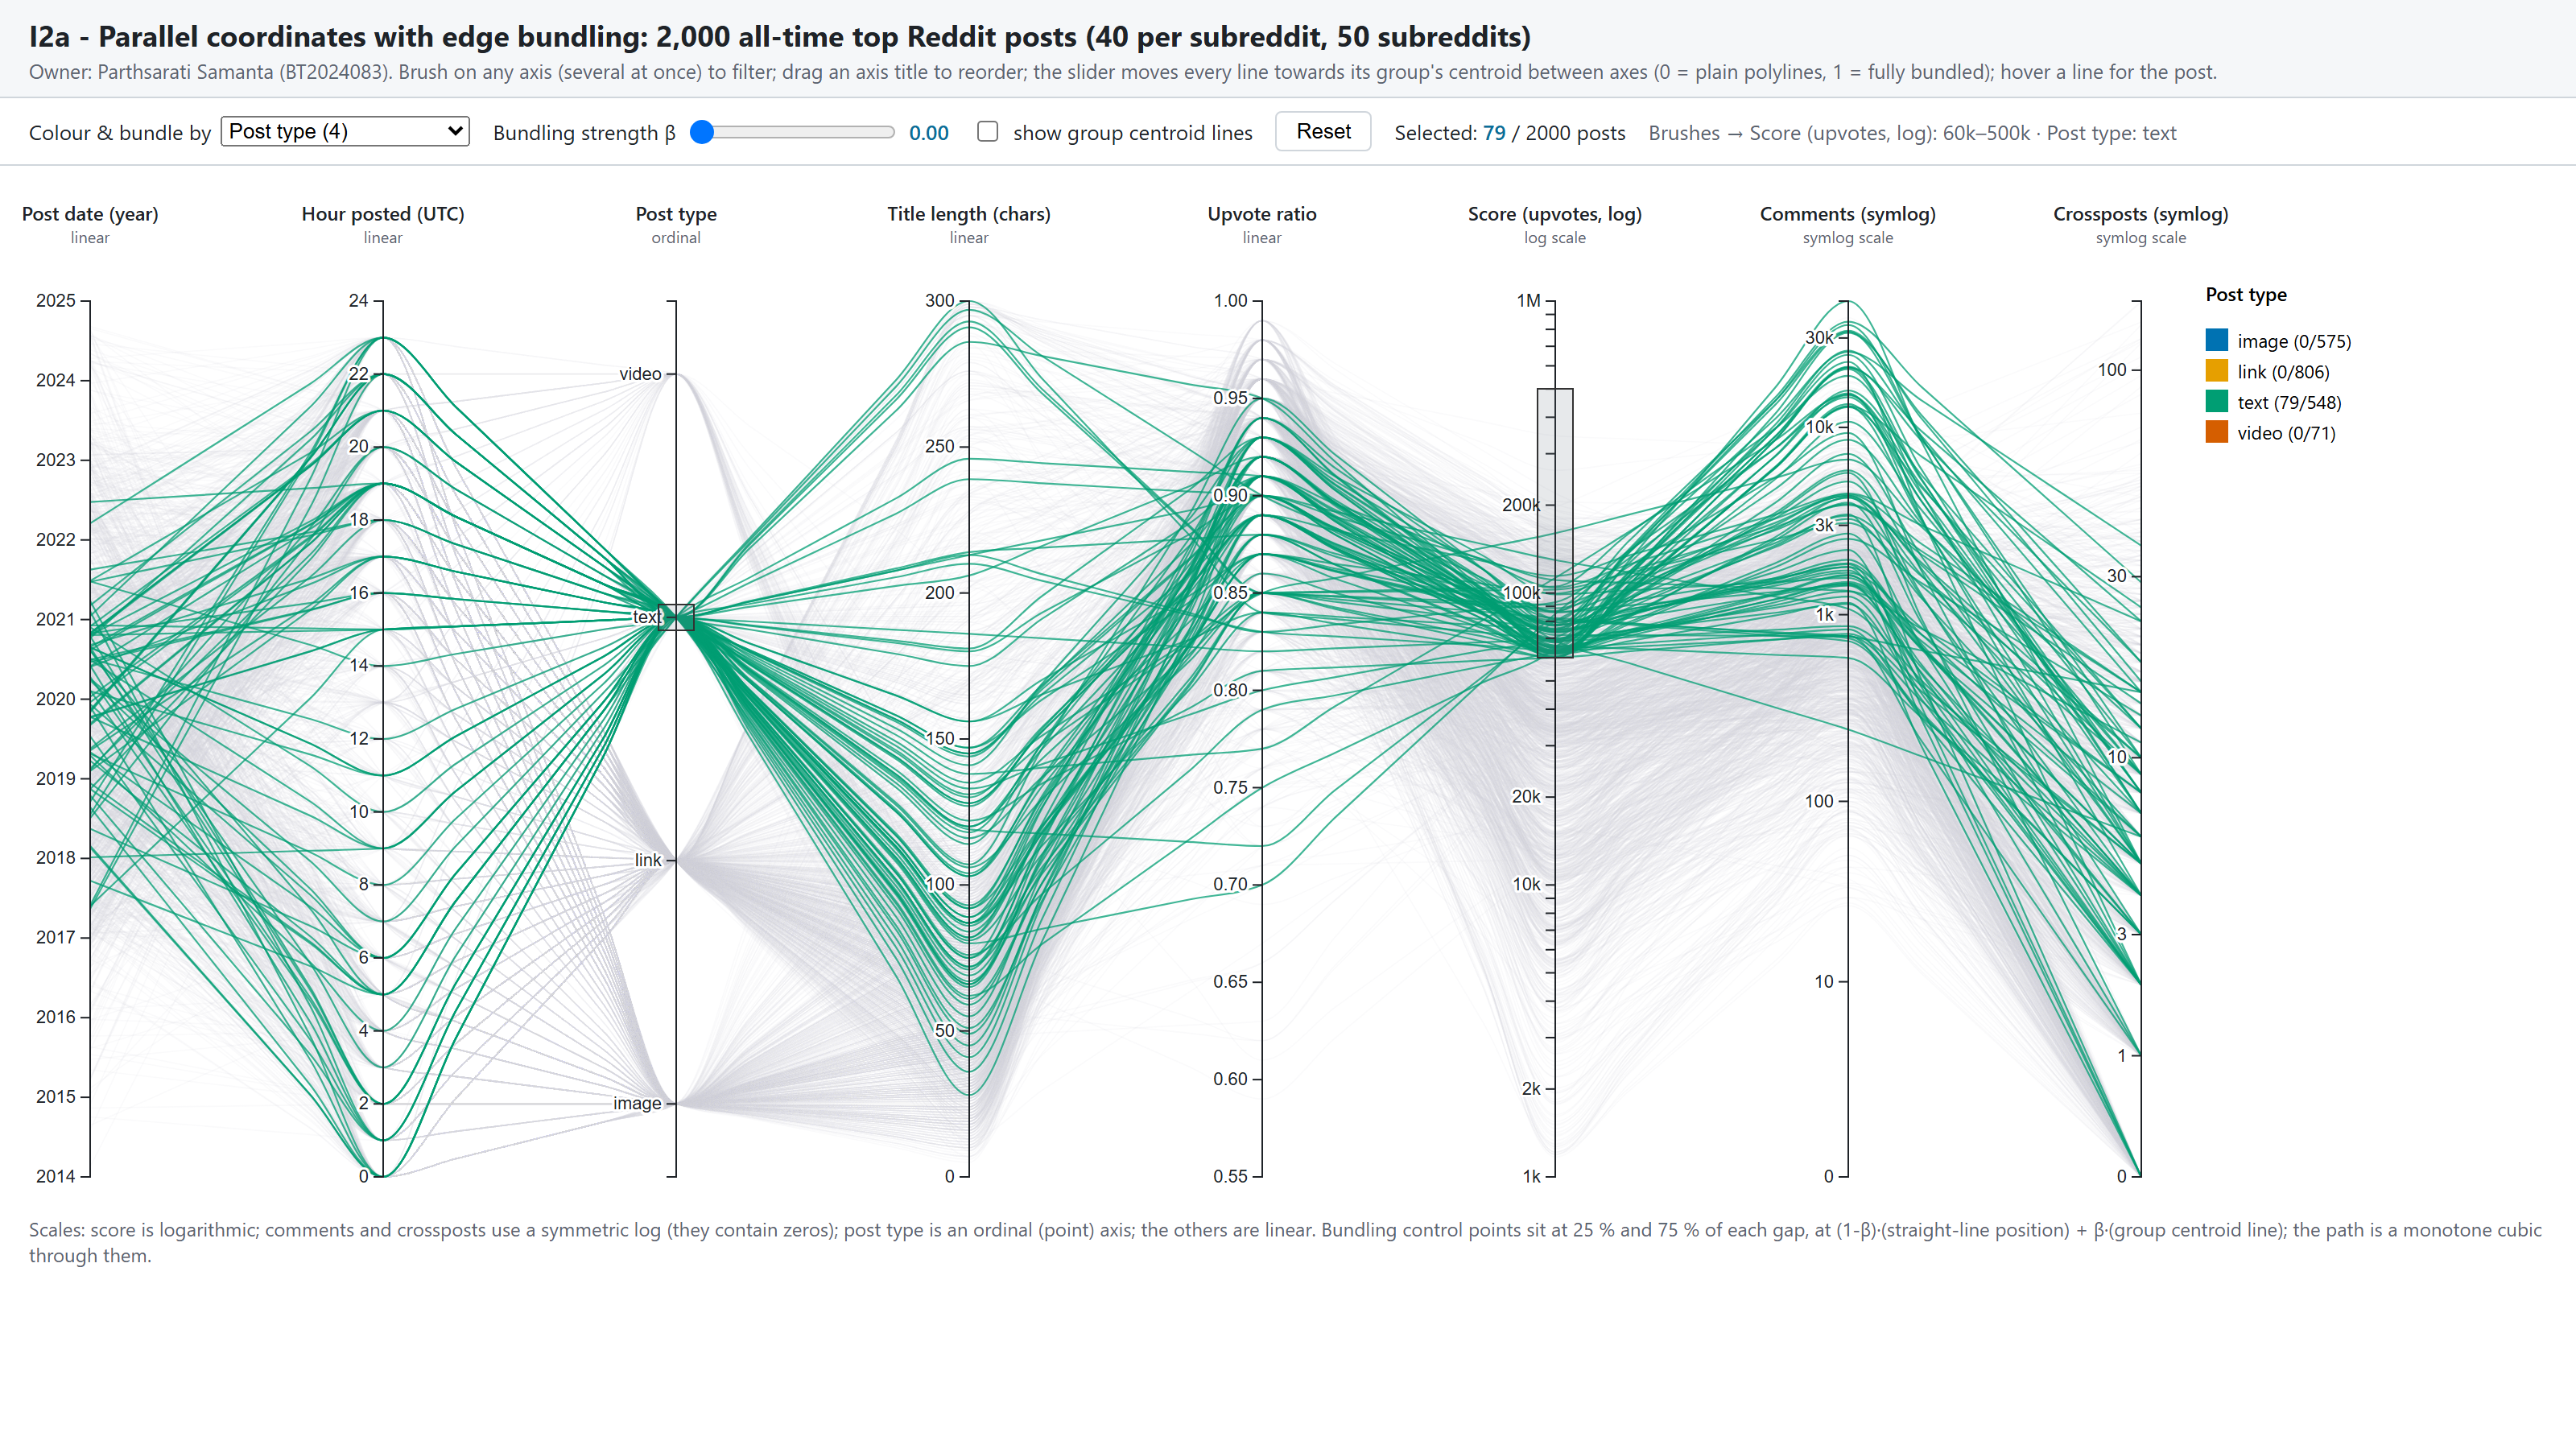
\includegraphics[width=0.495\textwidth]{Fig_32a_parcoords_brush_score_text.png}}\hfill
\subfloat[Brushes: comments $\ge$3,000 AND upvote ratio $\le$0.85; colour = topic]{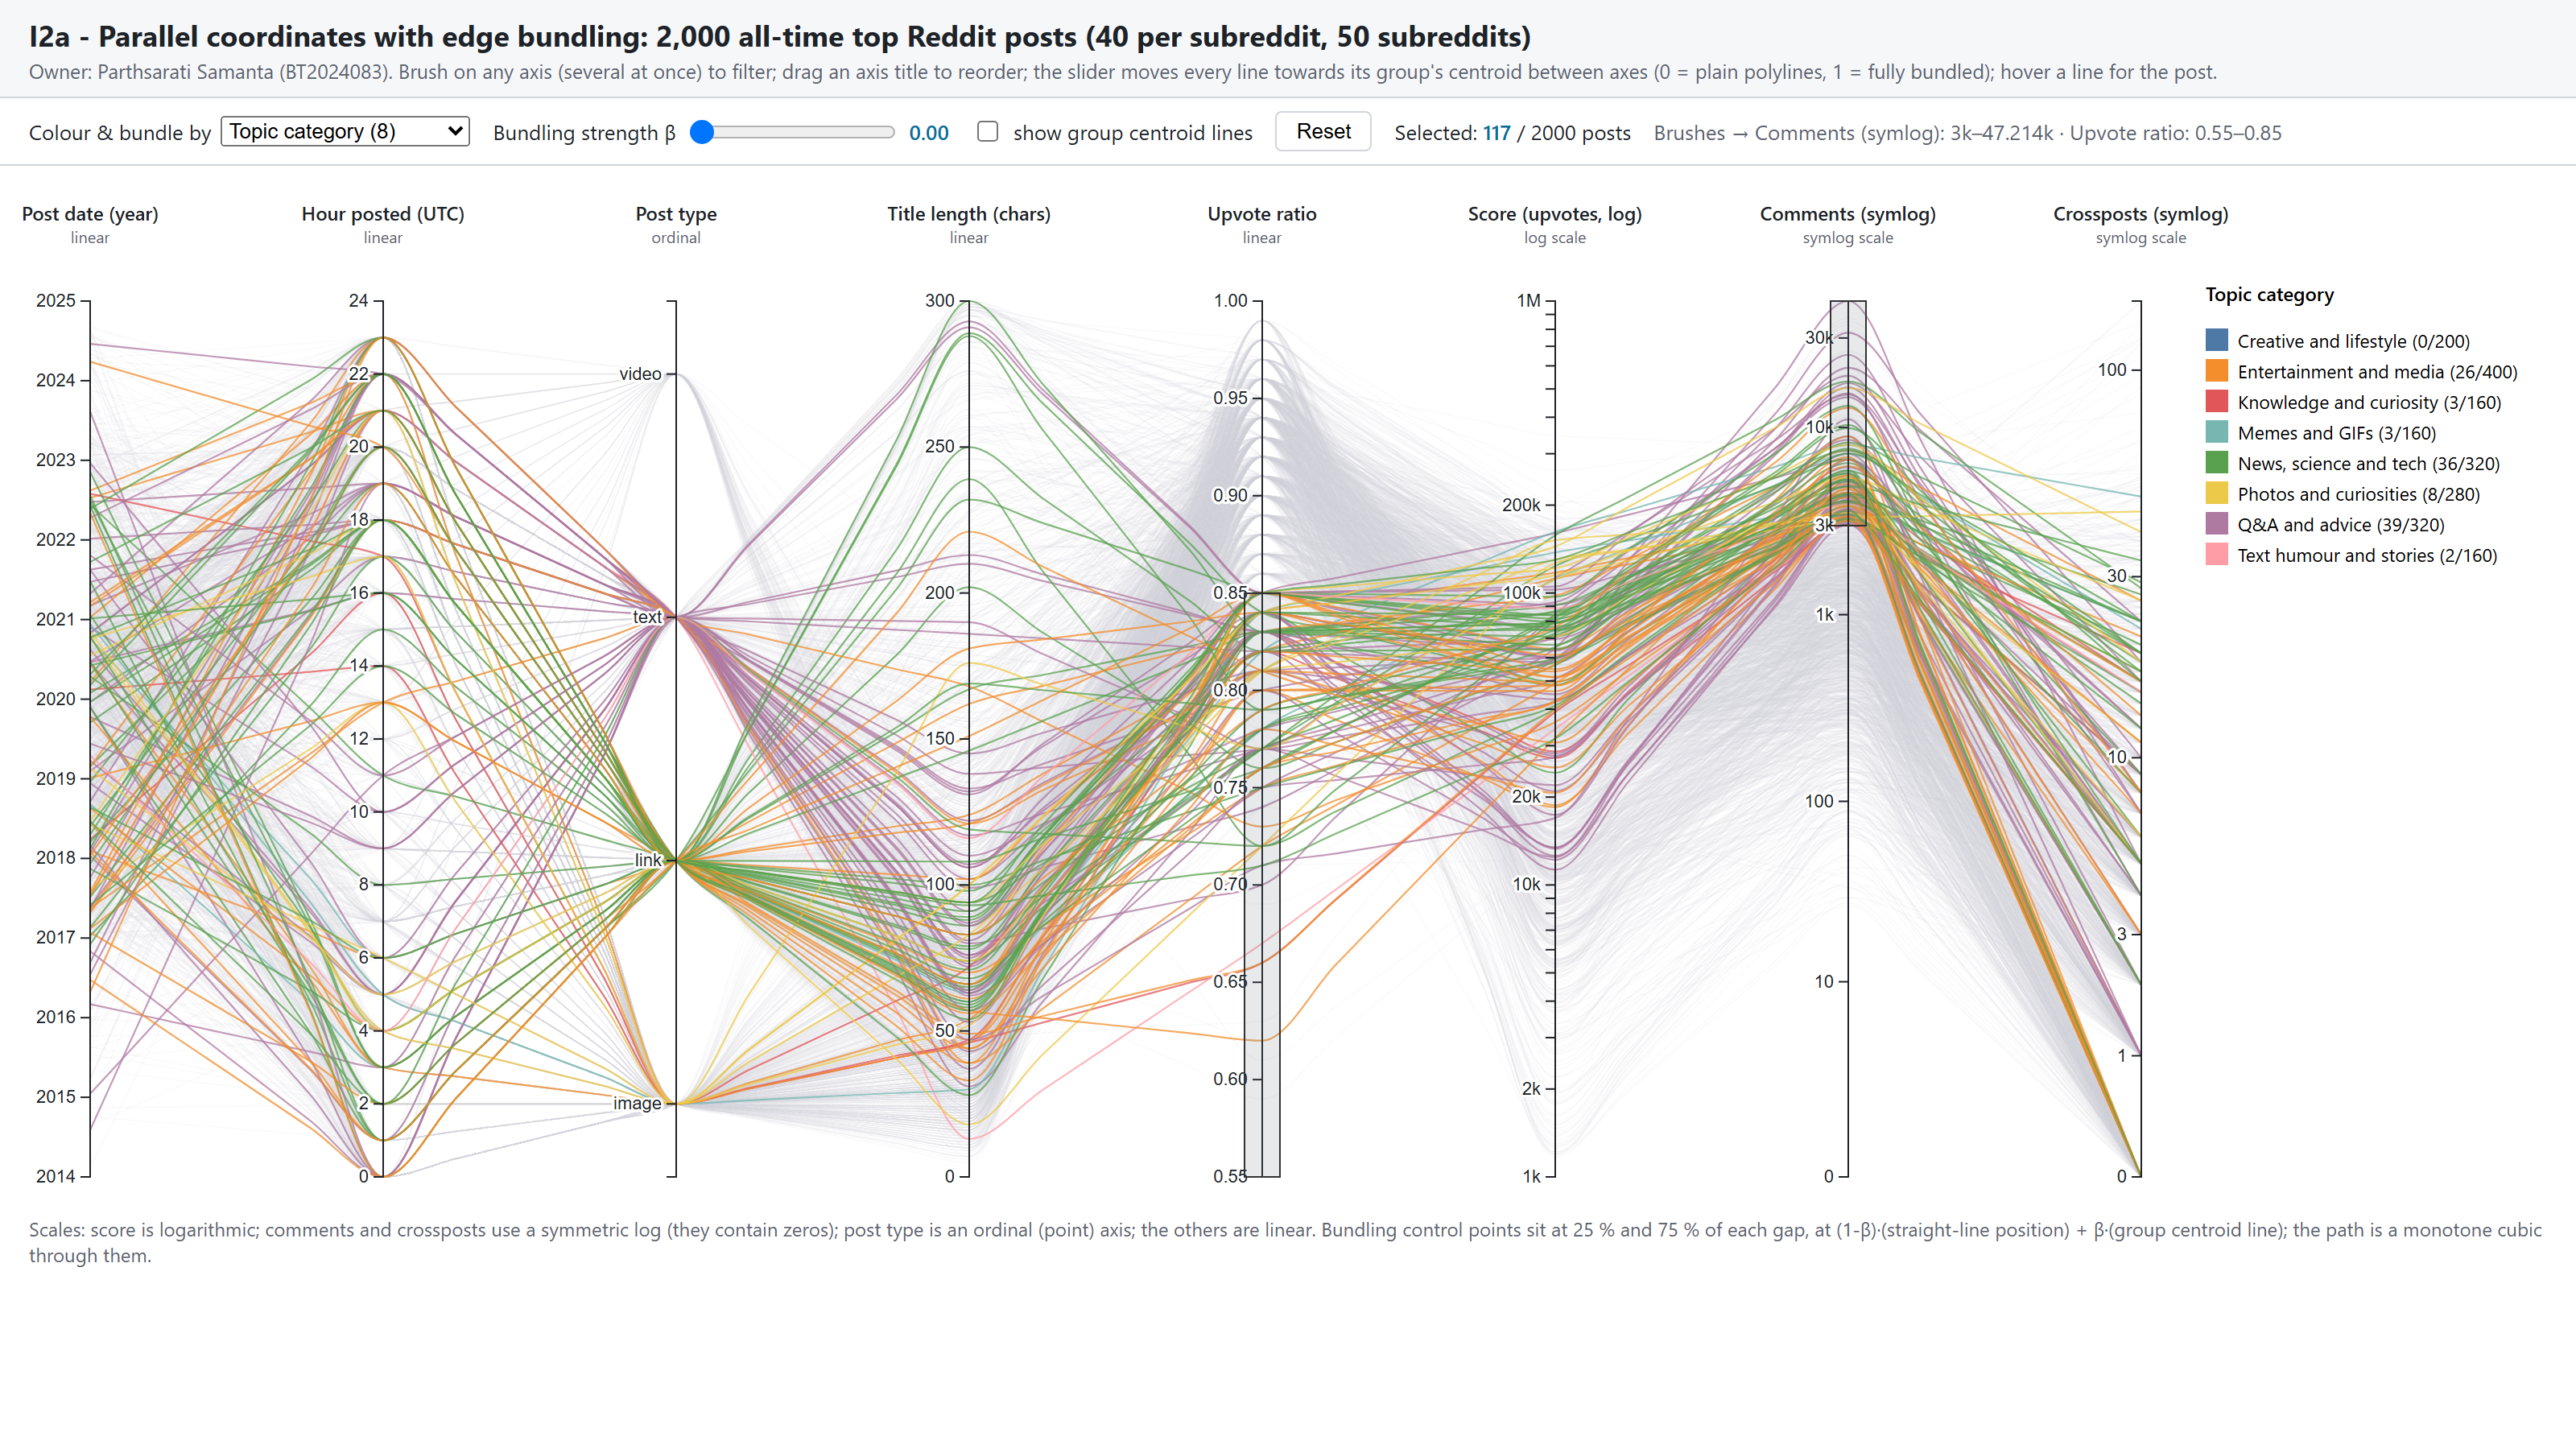
\includegraphics[width=0.495\textwidth]{Fig_32b_parcoords_brush_controversial.png}}\\
\subfloat[Axes reordered (post type first, date last), $\beta=0.5$, brush year $\ge$2021]{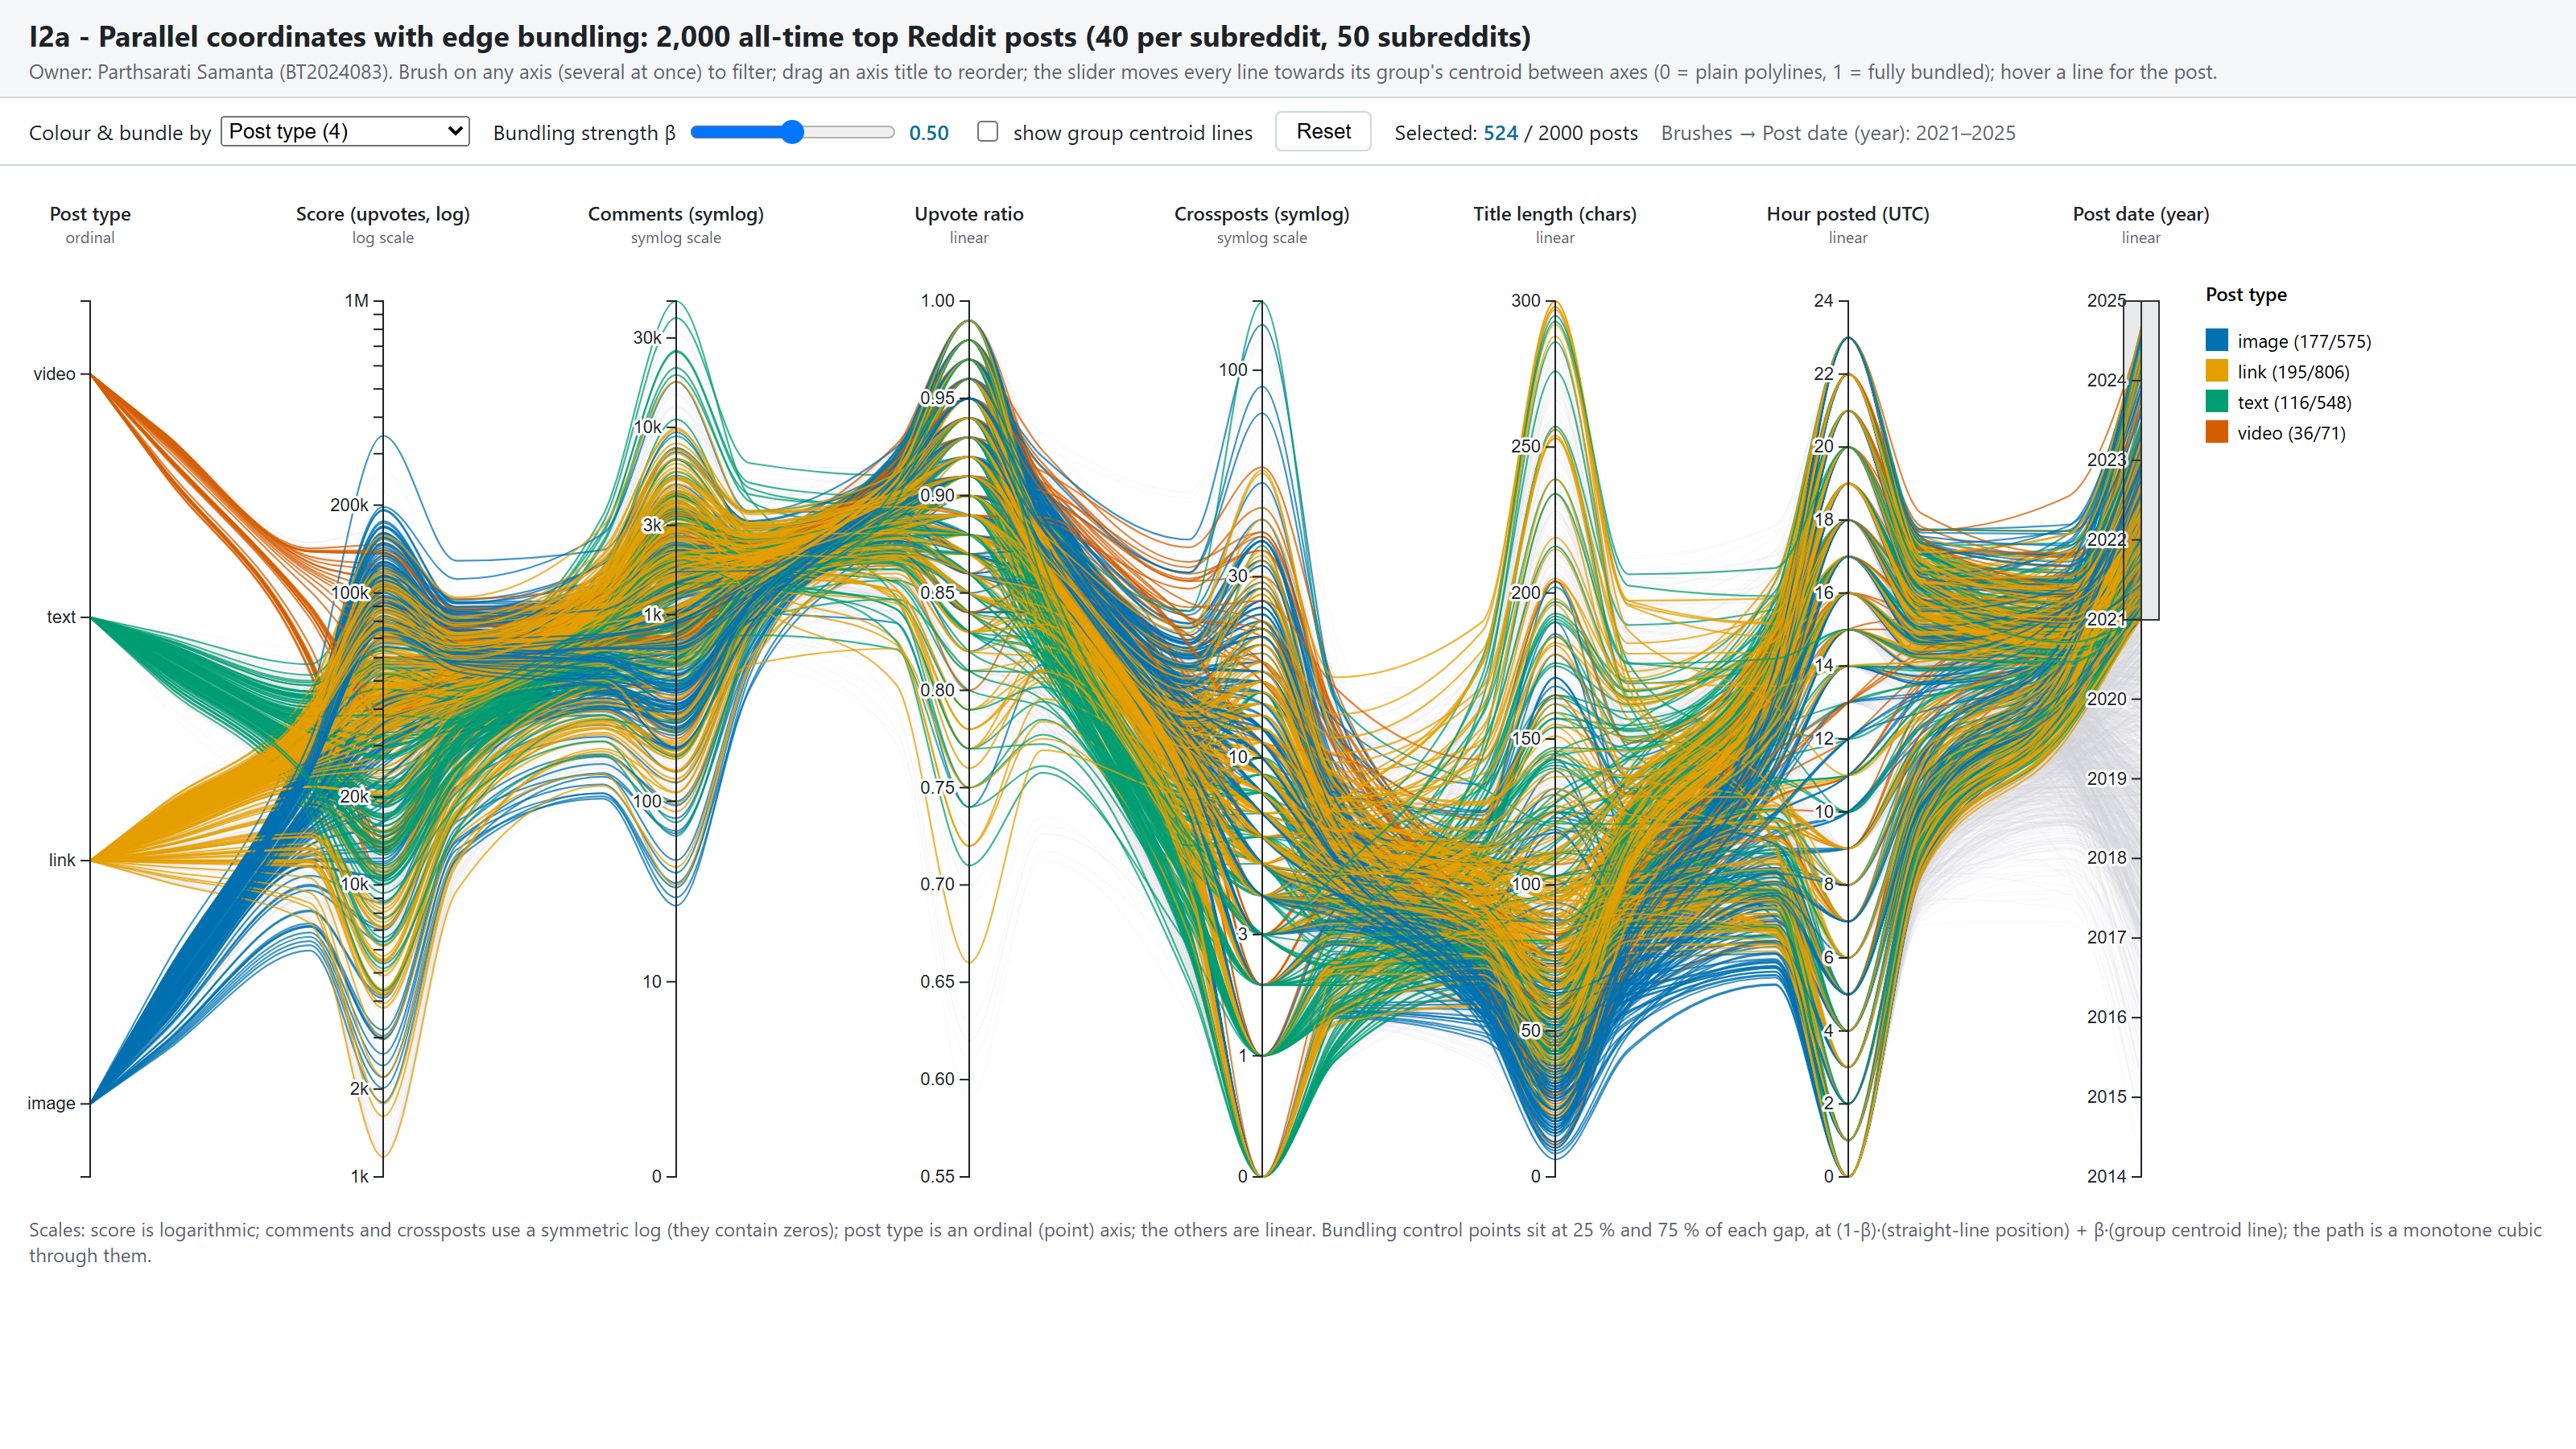
\includegraphics[width=0.495\textwidth]{Fig_32c_parcoords_reordered.png}}
\caption{Brushing and axis reordering (I2a). Files \fpath{Fig_32a/b/c_*.png}.}
\label{fig:32}
\end{figure*}

\input{generated/tab_pcstates}

\textbf{Inferences (bundling, Fig.~\ref{fig:31}).}
(1) Unbundled (Fig.~\ref{fig:31}a), 2,000 lines over eight axes form a dense ``hairball''. Only marginal patterns are
visible: hours cluster at 14--23 and 0--5 UTC (US daytime and evening), scores span 1k--400k, and most upvote ratios sit at
0.85--0.97.
(2) Bundling with $\beta=0.85$ (Fig.~\ref{fig:31}b) turns the four k-means clusters into four readable ribbons. C1 (675
posts) is the \emph{night-UTC} cluster (median hour 3 UTC, i.e.\ US evening) with medium score (median 43.9k). C2 (553) is
the \emph{high-performing evening} cluster (median hour 19 UTC, the highest median score 70.7k, 1,598 comments and 10
crossposts). C0 (552) has the same evening hours but is \emph{low-reach} (median score 14.9k, 0 crossposts). C3 (220) is
the \emph{long-title} cluster (median title of 242 characters against about 65 elsewhere), mostly link and text posts.
Hour and crossposts, not topic, drive the clustering. That explains the low silhouette (0.248): the clusters are bands in a
continuum.
(3) Bundling by topic (Fig.~\ref{fig:31}c) with centroid lines shows that Q\&A and text communities sit at the
\emph{text} position of the post-type axis with low crossposts, while image communities (Photos, Memes) have the highest
centroid scores. Ribbon crossings between axes show negative relations, such as upvote ratio against comments.
(4) The cost of bundling is fidelity between axes. At high $\beta$ the line segments between two axes no longer show the
individual pairwise relation, and outliers within a group are pulled into the ribbon. We therefore keep the slider
and read individual records at $\beta=0$.

\textbf{Inferences (brushing and reordering, Fig.~\ref{fig:32}, Table~\ref{tab:pcstates}).}
(1) Brushing score $\ge$60k selects 654 posts (33\,\%): link 276, image 262, text 79, video 37. Adding post type = text
leaves 79 posts, of which 32 are from AskReddit, 27 from Showerthoughts and 9 from LifeProTips (Fig.~\ref{fig:32}a). Text
posts reach the very top almost only in three ``prompt'' communities, and their titles are short (Showerthoughts and
AskReddit questions).
(2) Brushing comments $\ge$3,000 \emph{and} upvote ratio $\le$0.85 isolates 117 \emph{controversial discussions} (median
ratio 0.82). They come from AskReddit (16), news (12), IAmA (11), videos (9) and Futurology (8). The brush shows the
negative association between agreement and discussion that the data confirm (Spearman $\rho=-0.45$ between upvote ratio
and comments): posts people argue about collect comments but fewer net upvotes.
(3) Reordering the axes to post type, score, comments, ratio, crossposts, title, hour, date (Fig.~\ref{fig:32}c) puts
related axes next to each other. Post type next to score shows that image and link posts dominate the top of the score
axis. Score next to comments shows a positive fan (Spearman 0.55). With year $\ge$2021 brushed on the now-rightmost date
axis, the 524 recent posts are 6.9\,\% video against 3.6\,\% overall, and 33.8\,\% image against 28.8\,\%, while text falls to
22.1\,\% from 27.4\,\%. This is the post-2020 shift towards native media, also seen in the treemap (Fig.~\ref{fig:33}).

\subsection{I2b: Zoomable treemap}
\textbf{Design.} We follow the zoomable-treemap pattern~\cite{shneiderman1992,bostock_zoomtreemap}. Every node's
children are laid out in the \emph{full viewport} with the chosen tiling and then scaled into the parent's rectangle. A
zoomed level therefore keeps the tiling's aspect-ratio behaviour at screen size (code in Appendix~\ref{app:code}).
\begin{itemize}
\item \emph{Zoom}: clicking a node zooms in with a 750\,ms transition; the breadcrumb or the header bar zooms out.
\item \emph{Next level}: thin white outlines show the next level inside each child.
\item \emph{Labels}: fitted (truncated with an ellipsis) and placed on opaque label plates so outlines never cross text.
\item \emph{Tooltips}: value, share of the parent and share of the whole.
\item \emph{Dropdowns}: three hierarchy remodels (H1--H3), three size measures (posts, total score, total comments), five
  tilings (squarify~\cite{bruls2000}, binary, slice, dice, slice-dice) and two sort orders (by size, by name).
\item \emph{Colour}: stable across remodels. Topic, post type, hosting class and era each have a fixed palette, years use
  viridis, and subreddits use shades of their topic colour.
\item \emph{Metrics line}: the mean, median and maximum aspect ratio of the current view, and the Kendall $\tau$ between
  the sort order and the reading order, as a measure of order preservation.
\end{itemize}

\begin{figure*}[!t]
\centering
\subfloat[H1 topic$\rightarrow$subreddit$\rightarrow$type, size = posts]{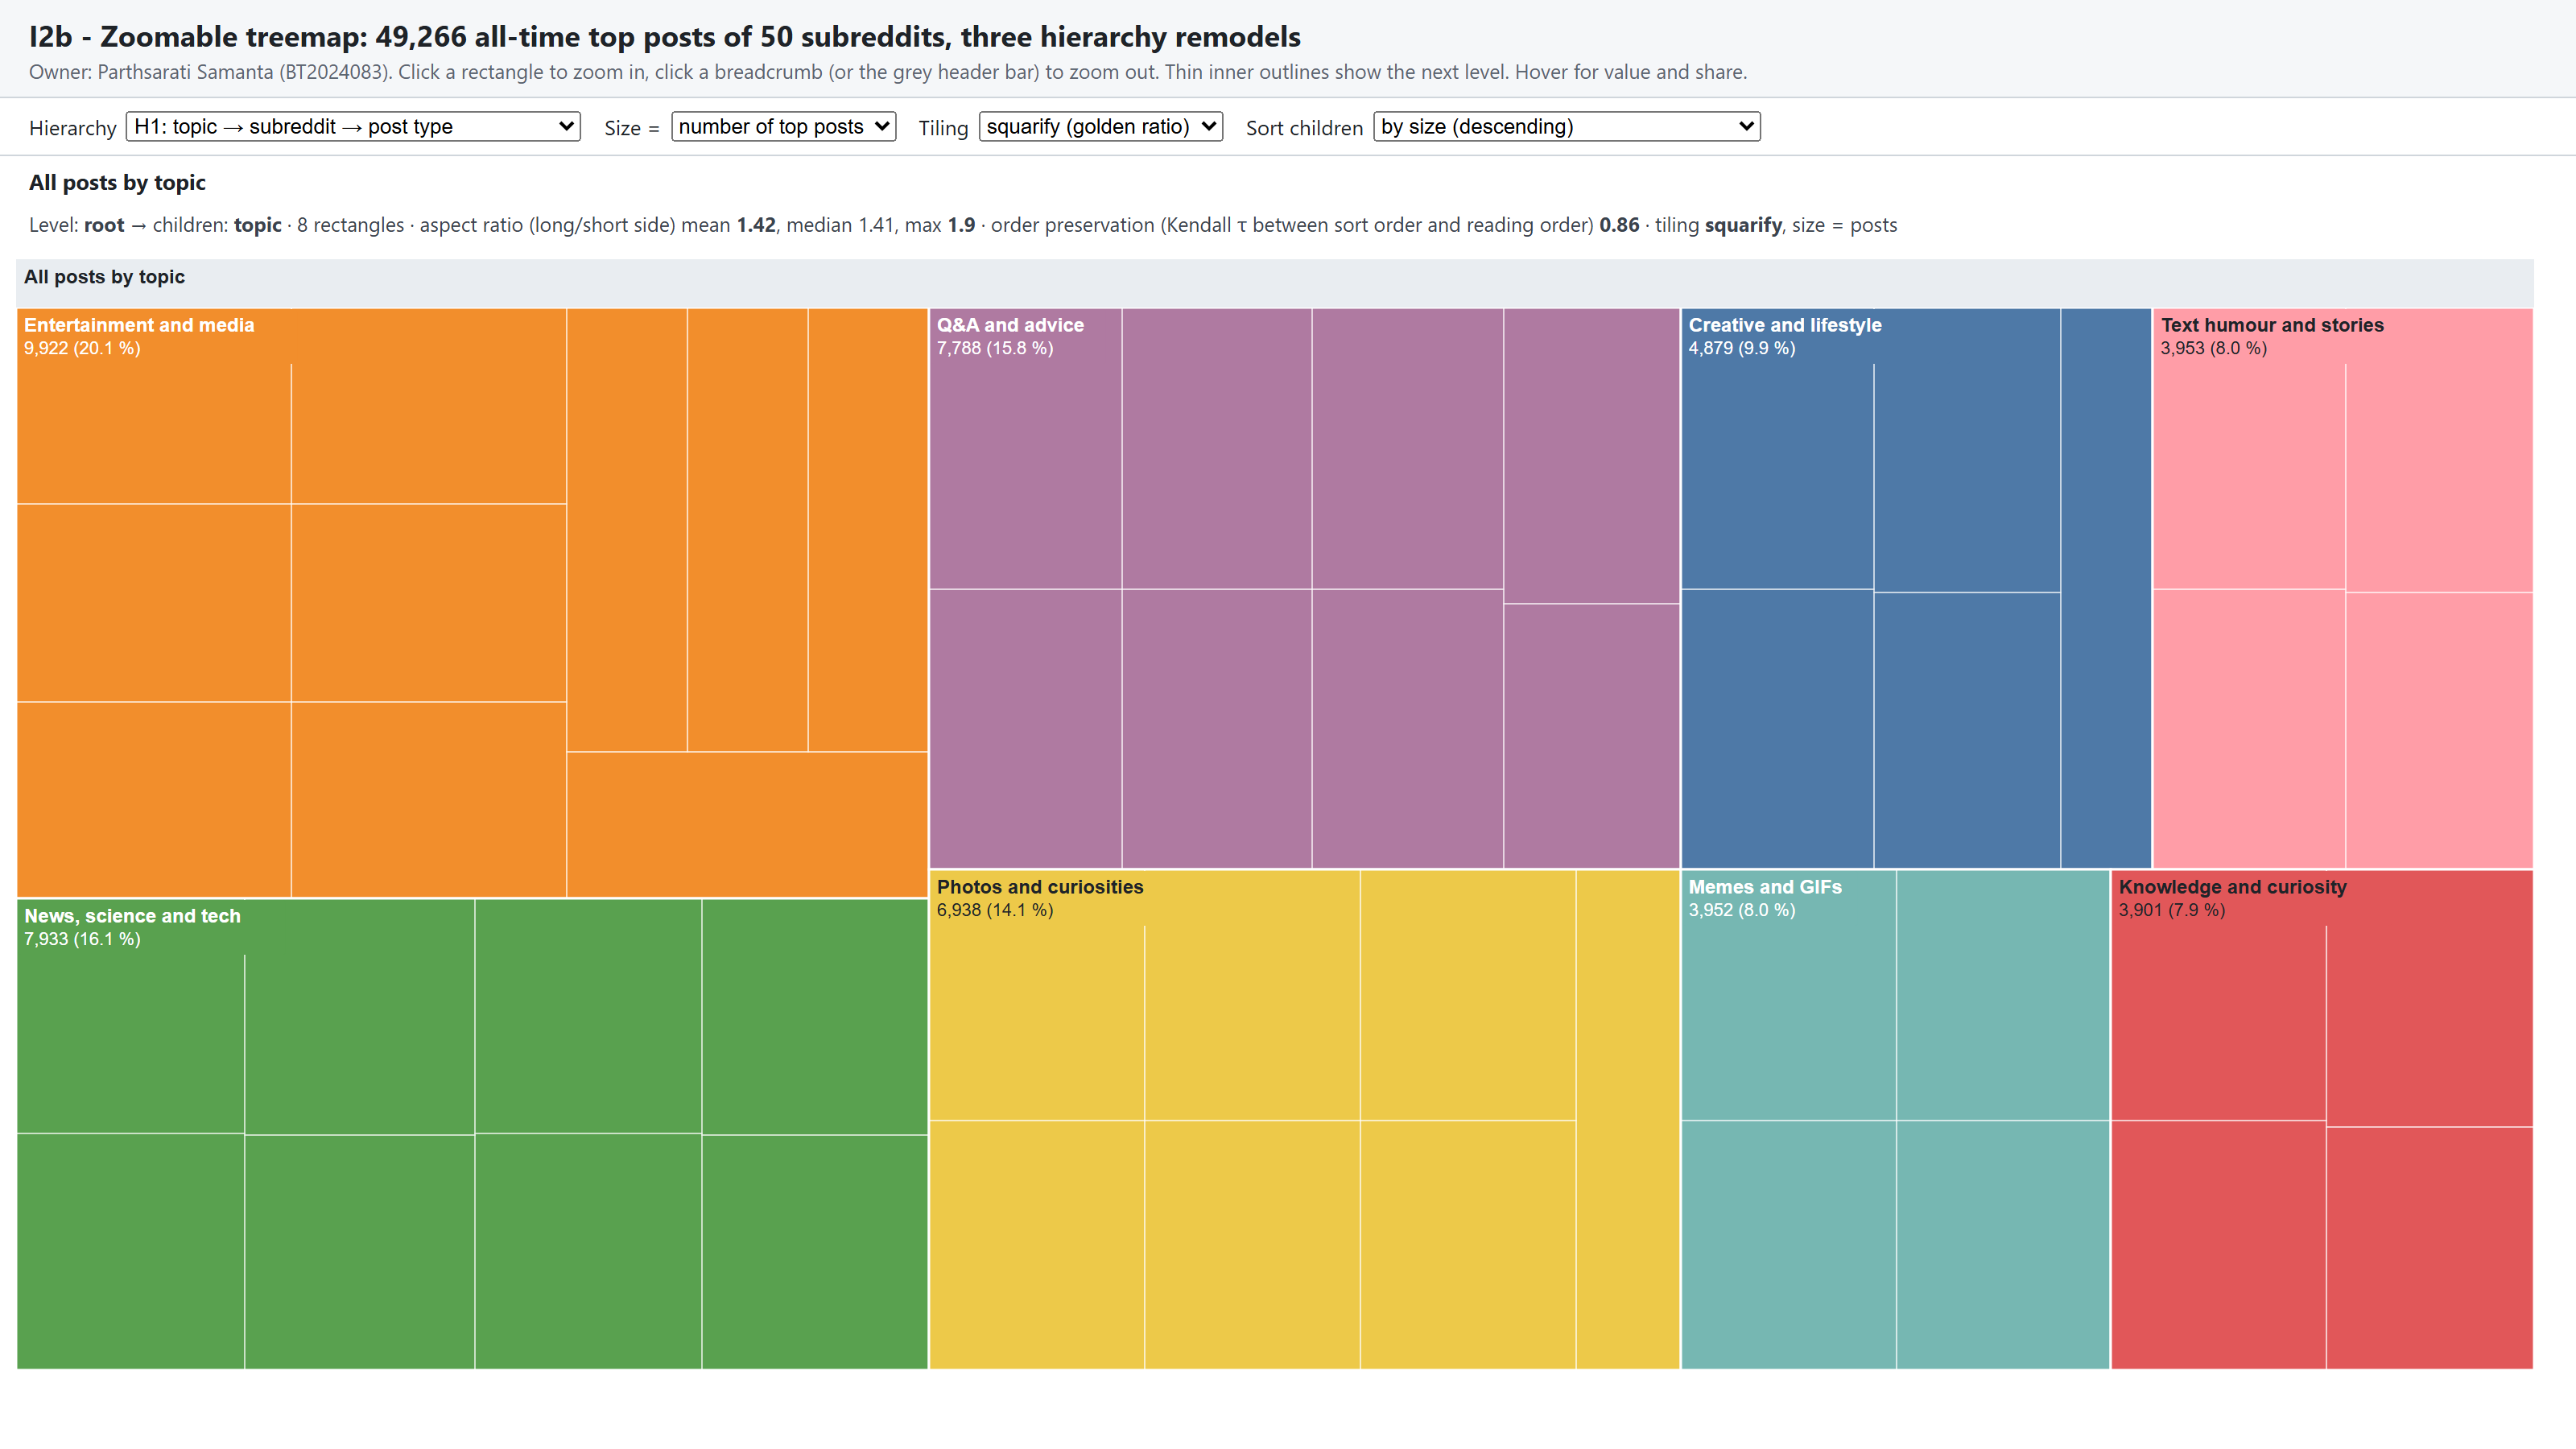
\includegraphics[width=0.495\textwidth]{Fig_33a_treemap_h1_topic.png}}\hfill
\subfloat[H2 post type$\rightarrow$hosting$\rightarrow$topic$\rightarrow$subreddit, size = posts]{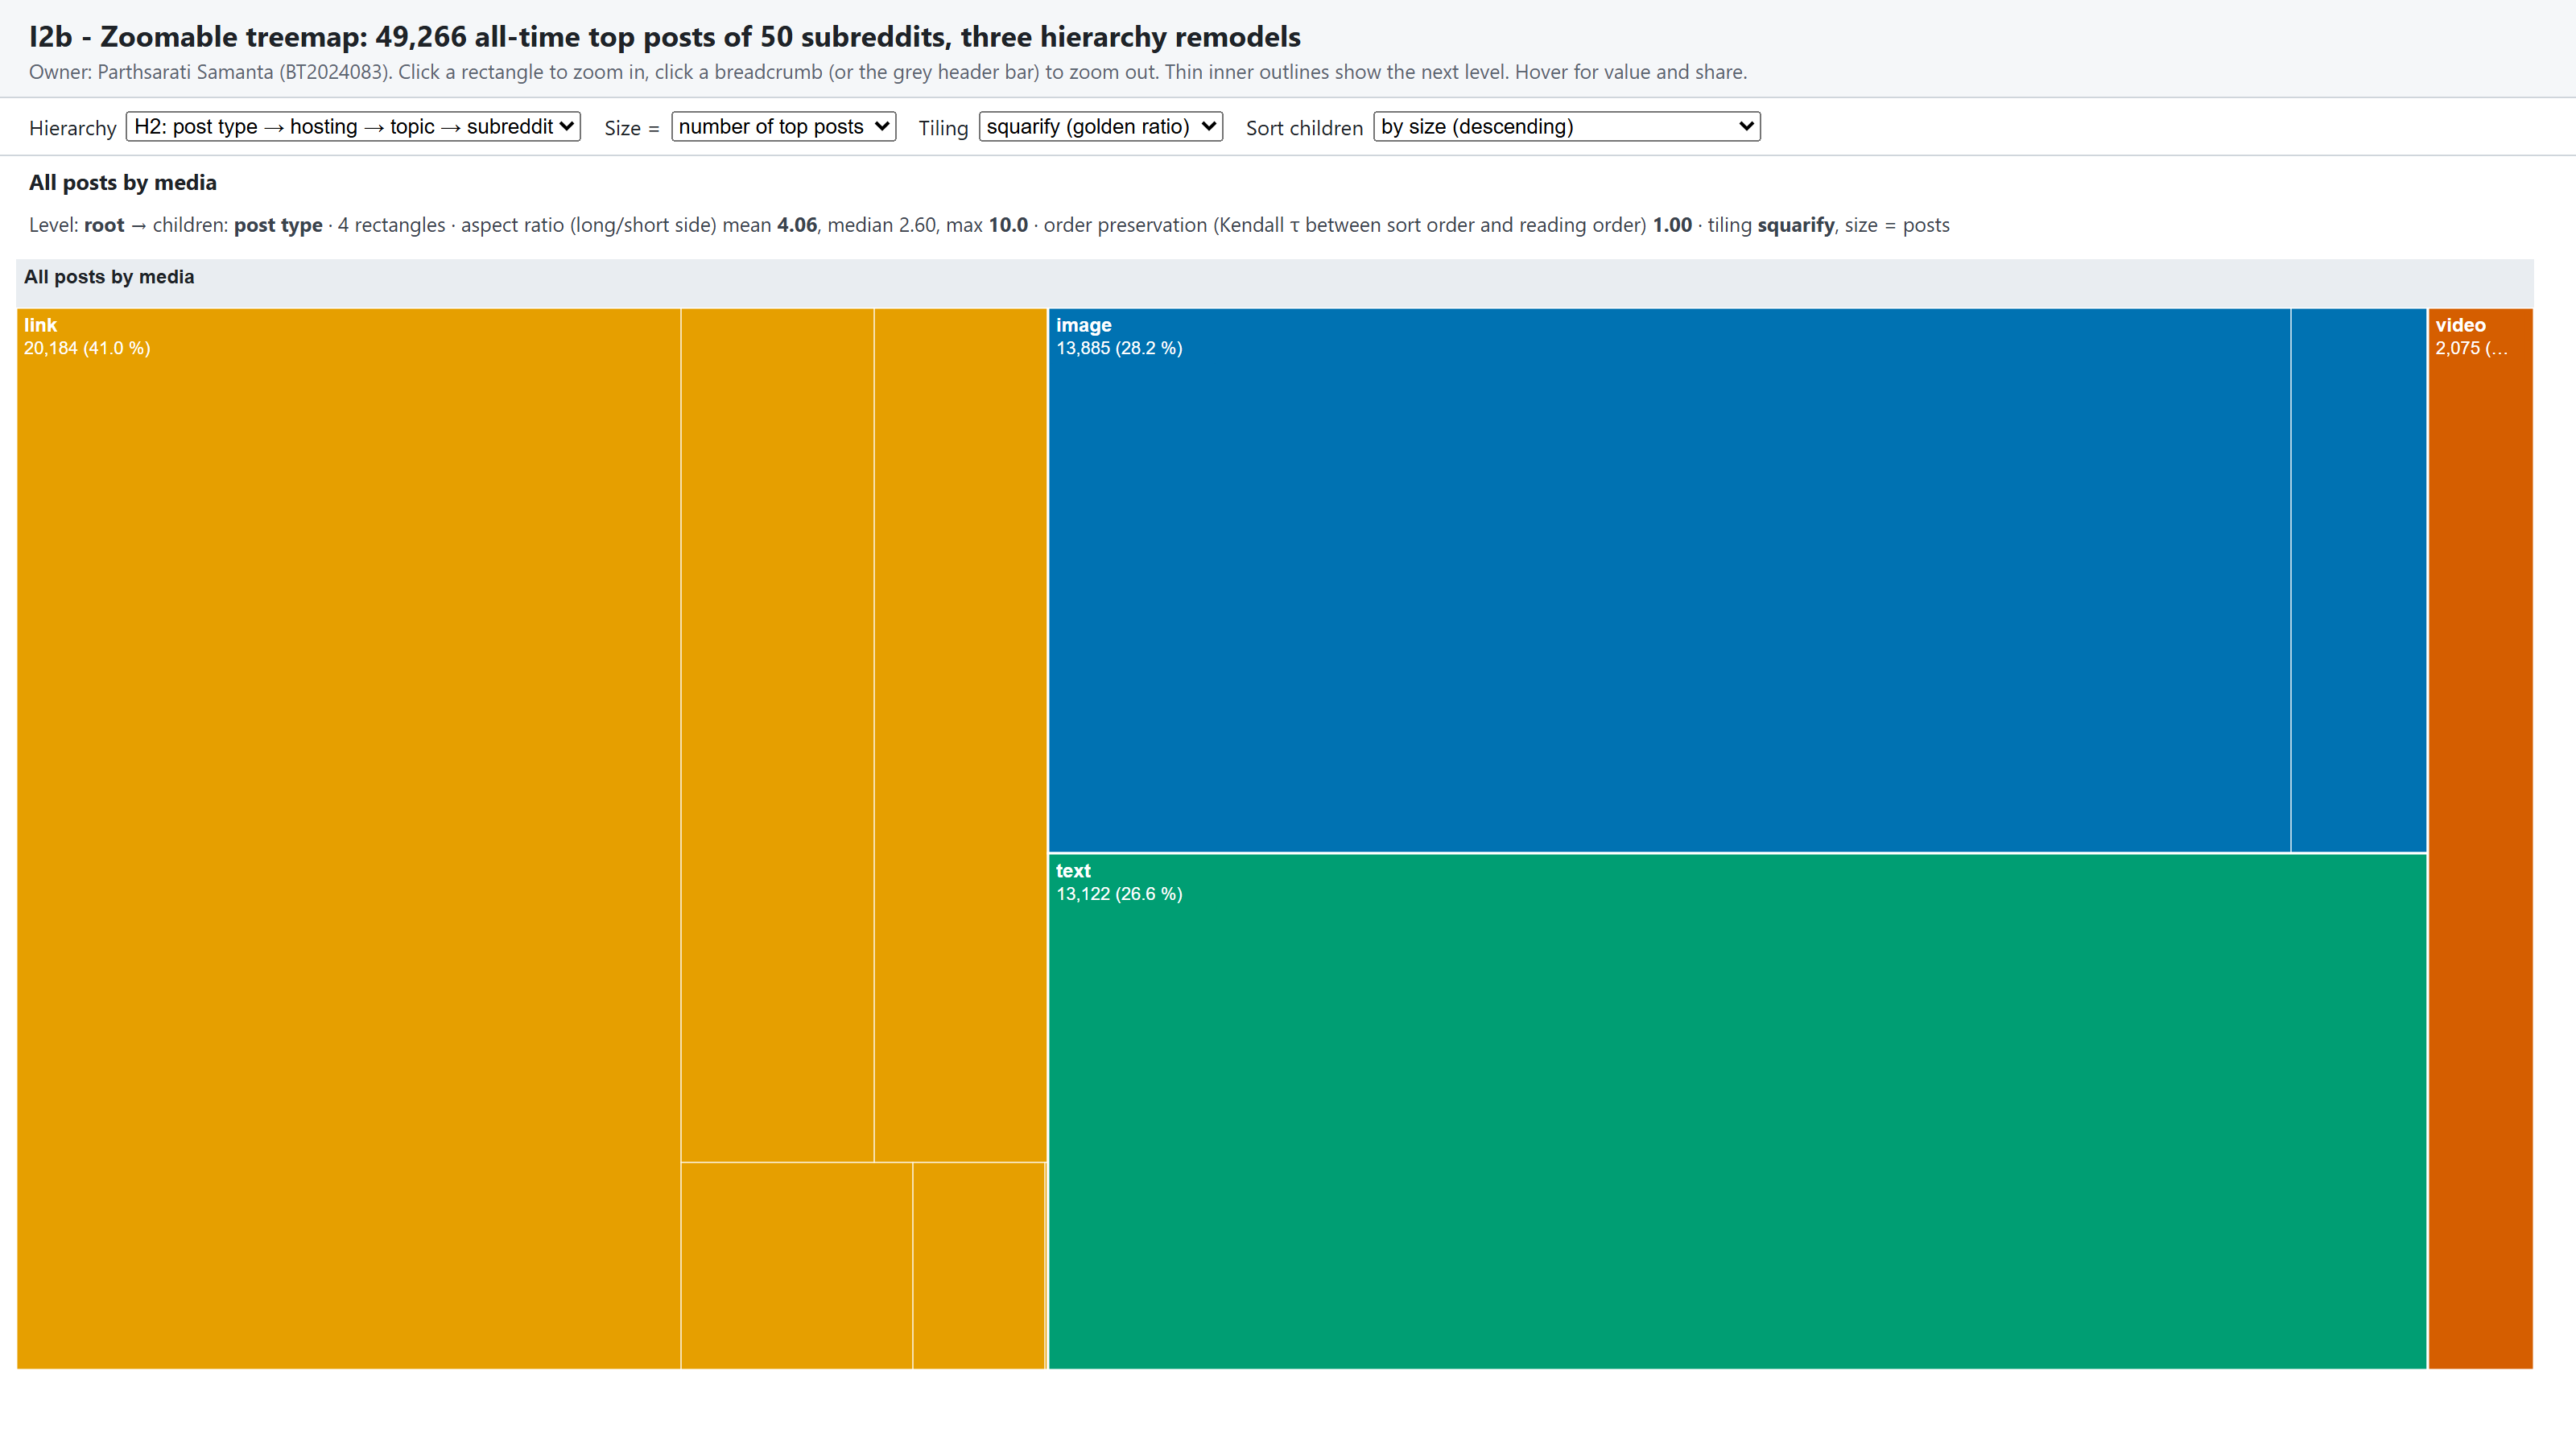
\includegraphics[width=0.495\textwidth]{Fig_33b_treemap_h2_media.png}}\\
\subfloat[H3 era$\rightarrow$year$\rightarrow$topic$\rightarrow$subreddit, size = posts]{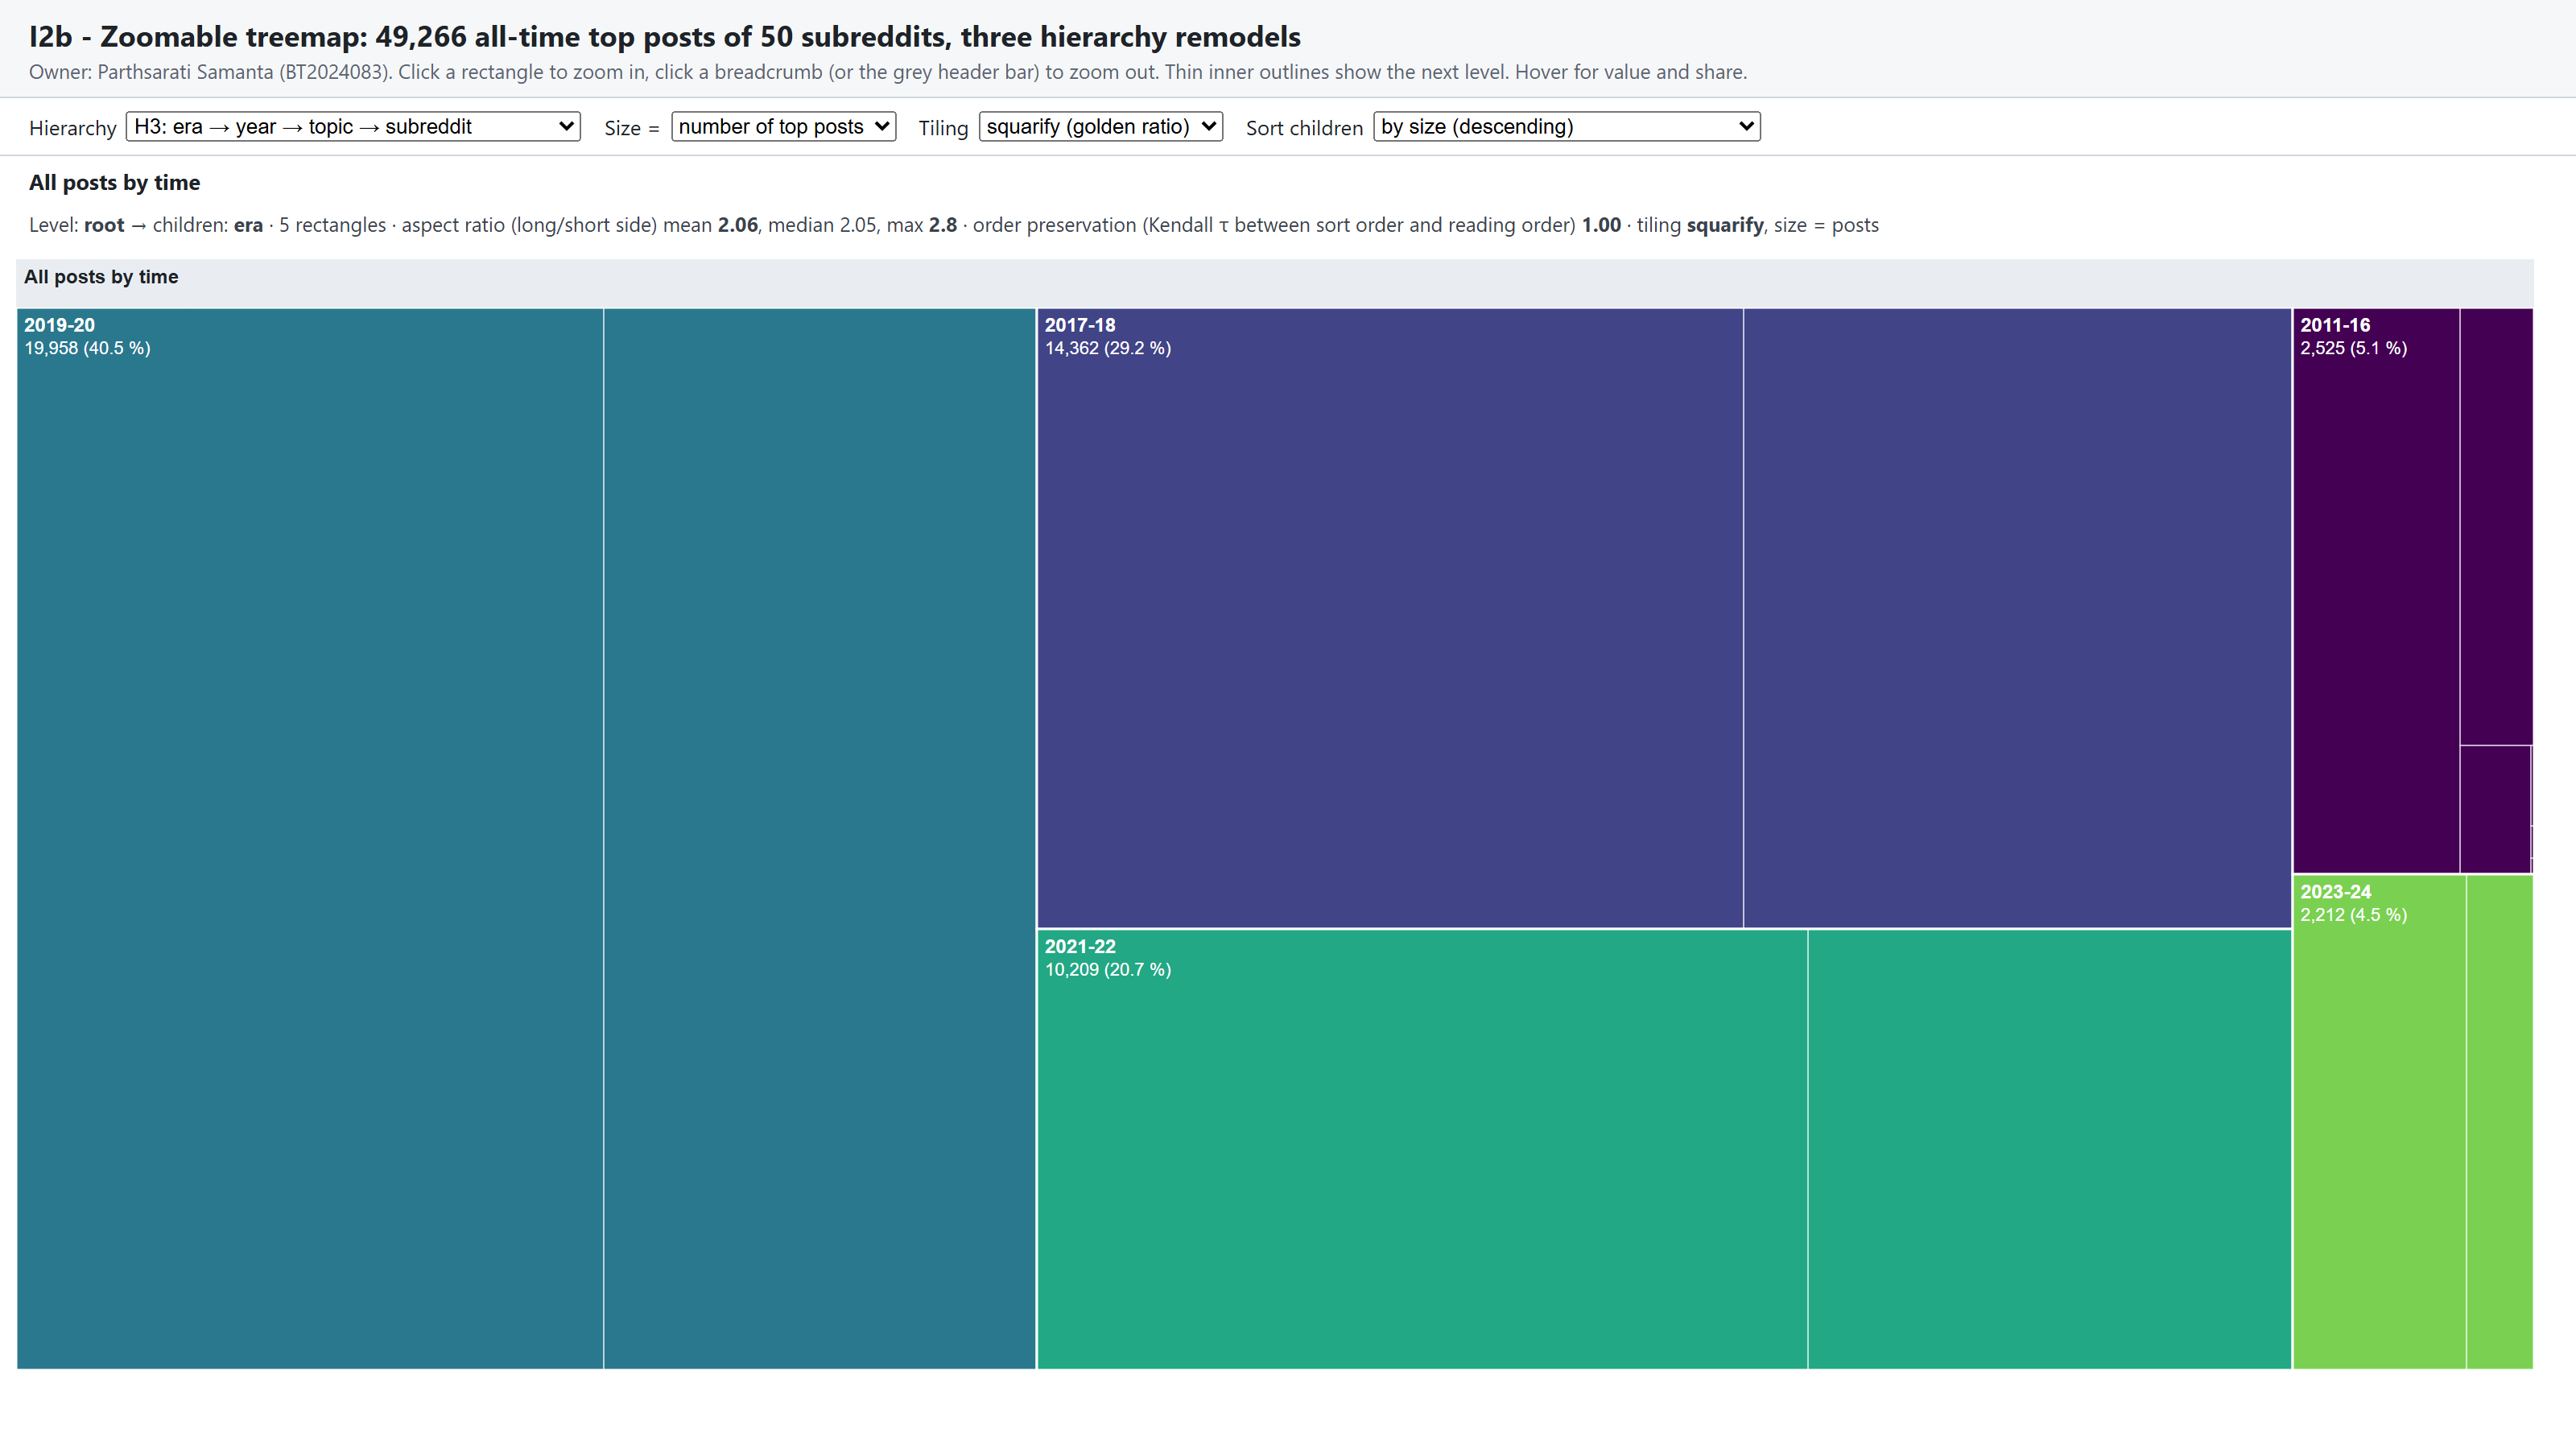
\includegraphics[width=0.495\textwidth]{Fig_33c_treemap_h3_time.png}}\hfill
\subfloat[H1 zoomed into Entertainment and media]{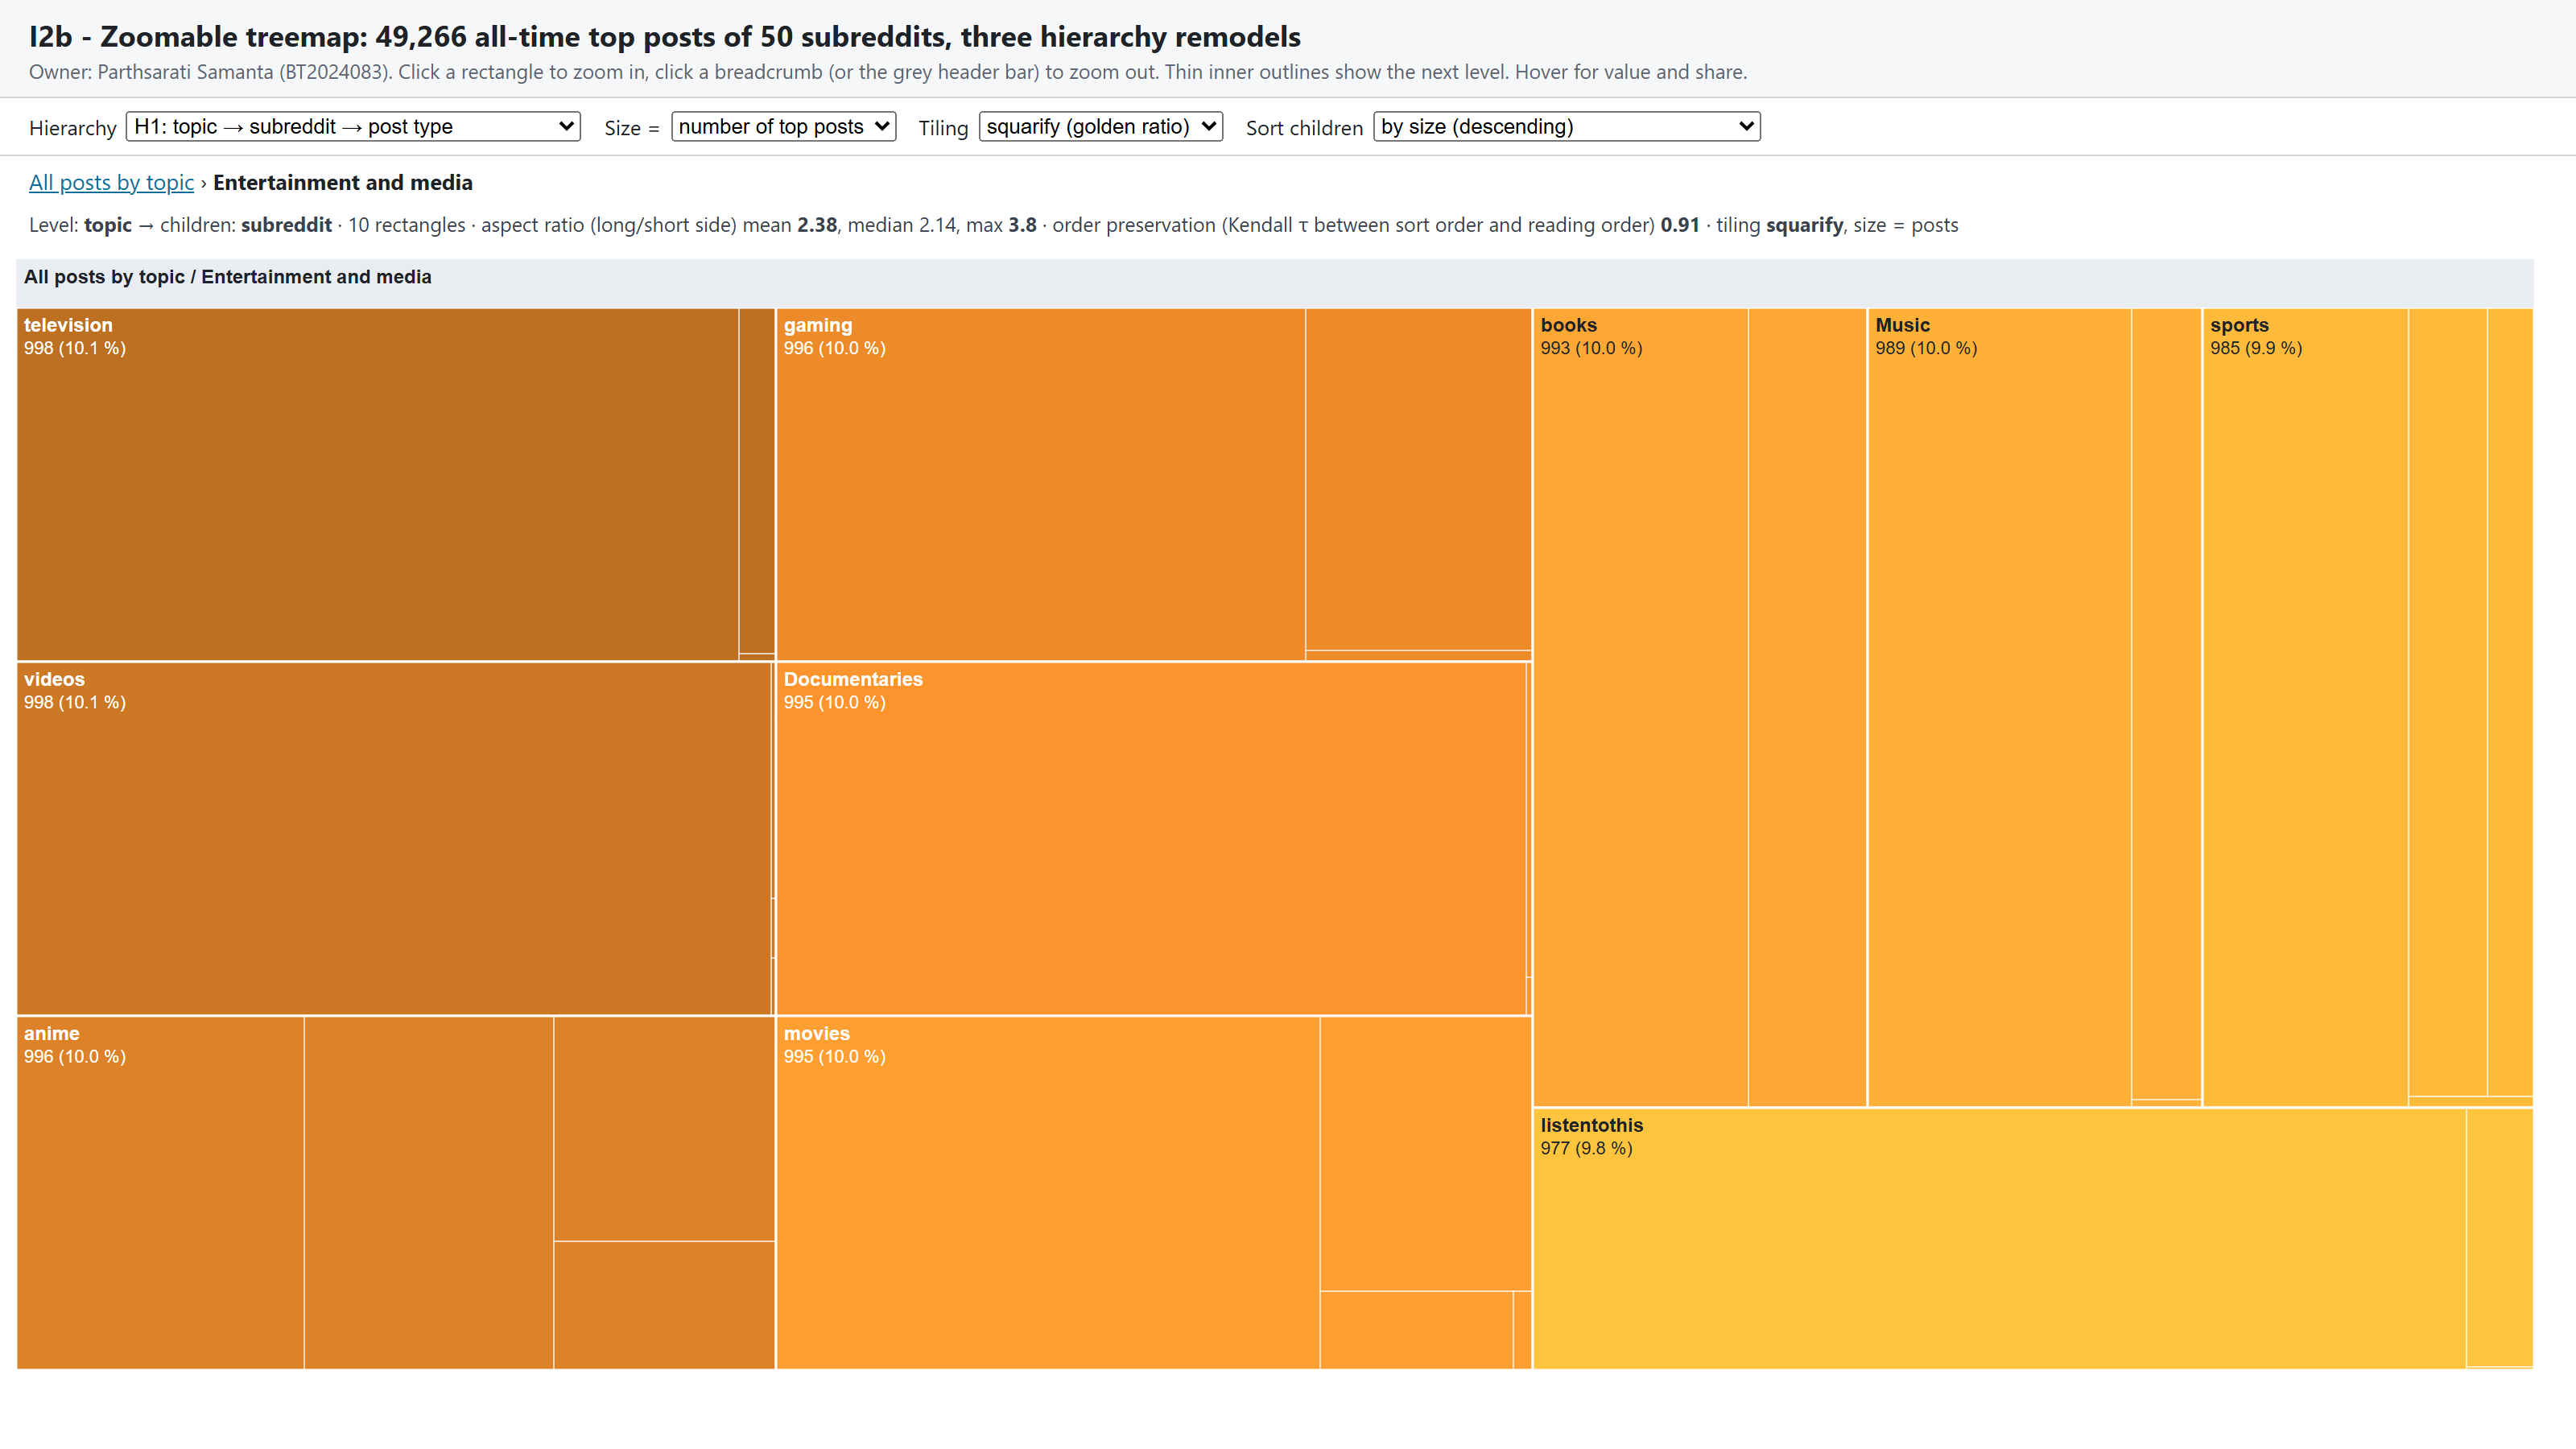
\includegraphics[width=0.495\textwidth]{Fig_33d_treemap_zoom_entertainment.png}}\\
\subfloat[H3 zoomed to 2019--20 / 2020, size = comments, sorted by name]{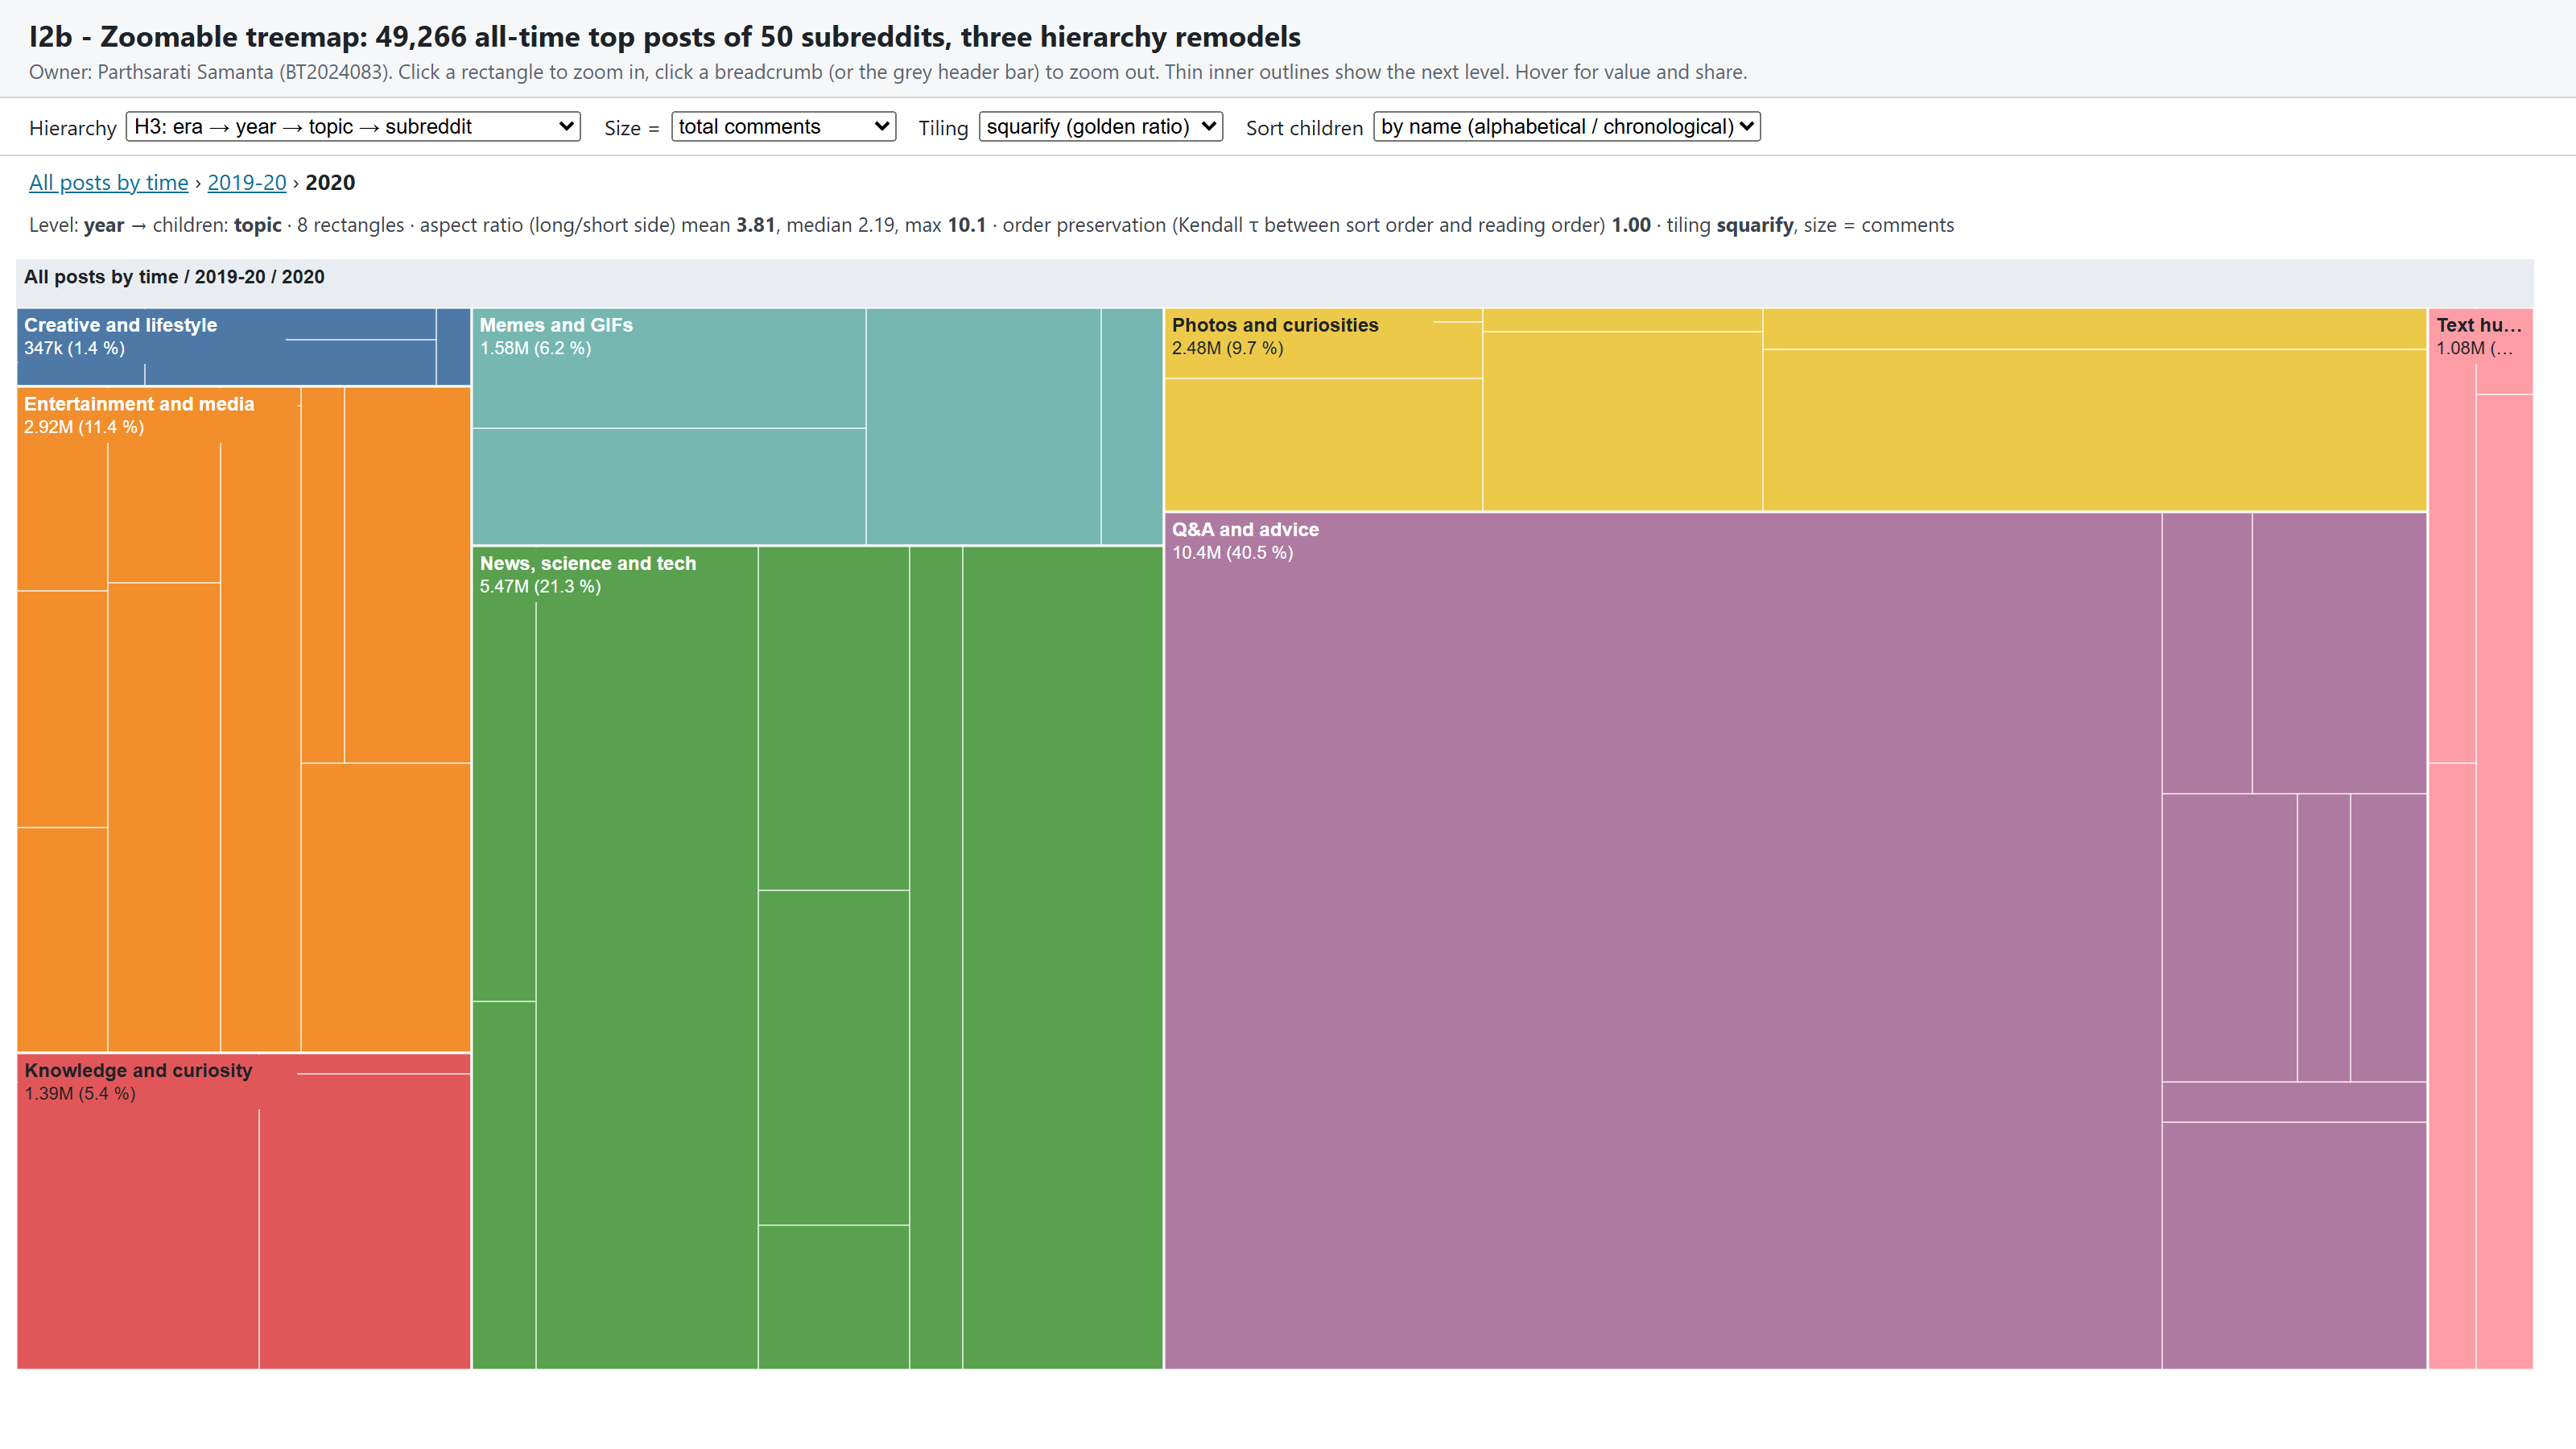
\includegraphics[width=0.495\textwidth]{Fig_33e_treemap_zoom_2020_comments.png}}\hfill
\subfloat[H2 zoomed into link posts, size = total score]{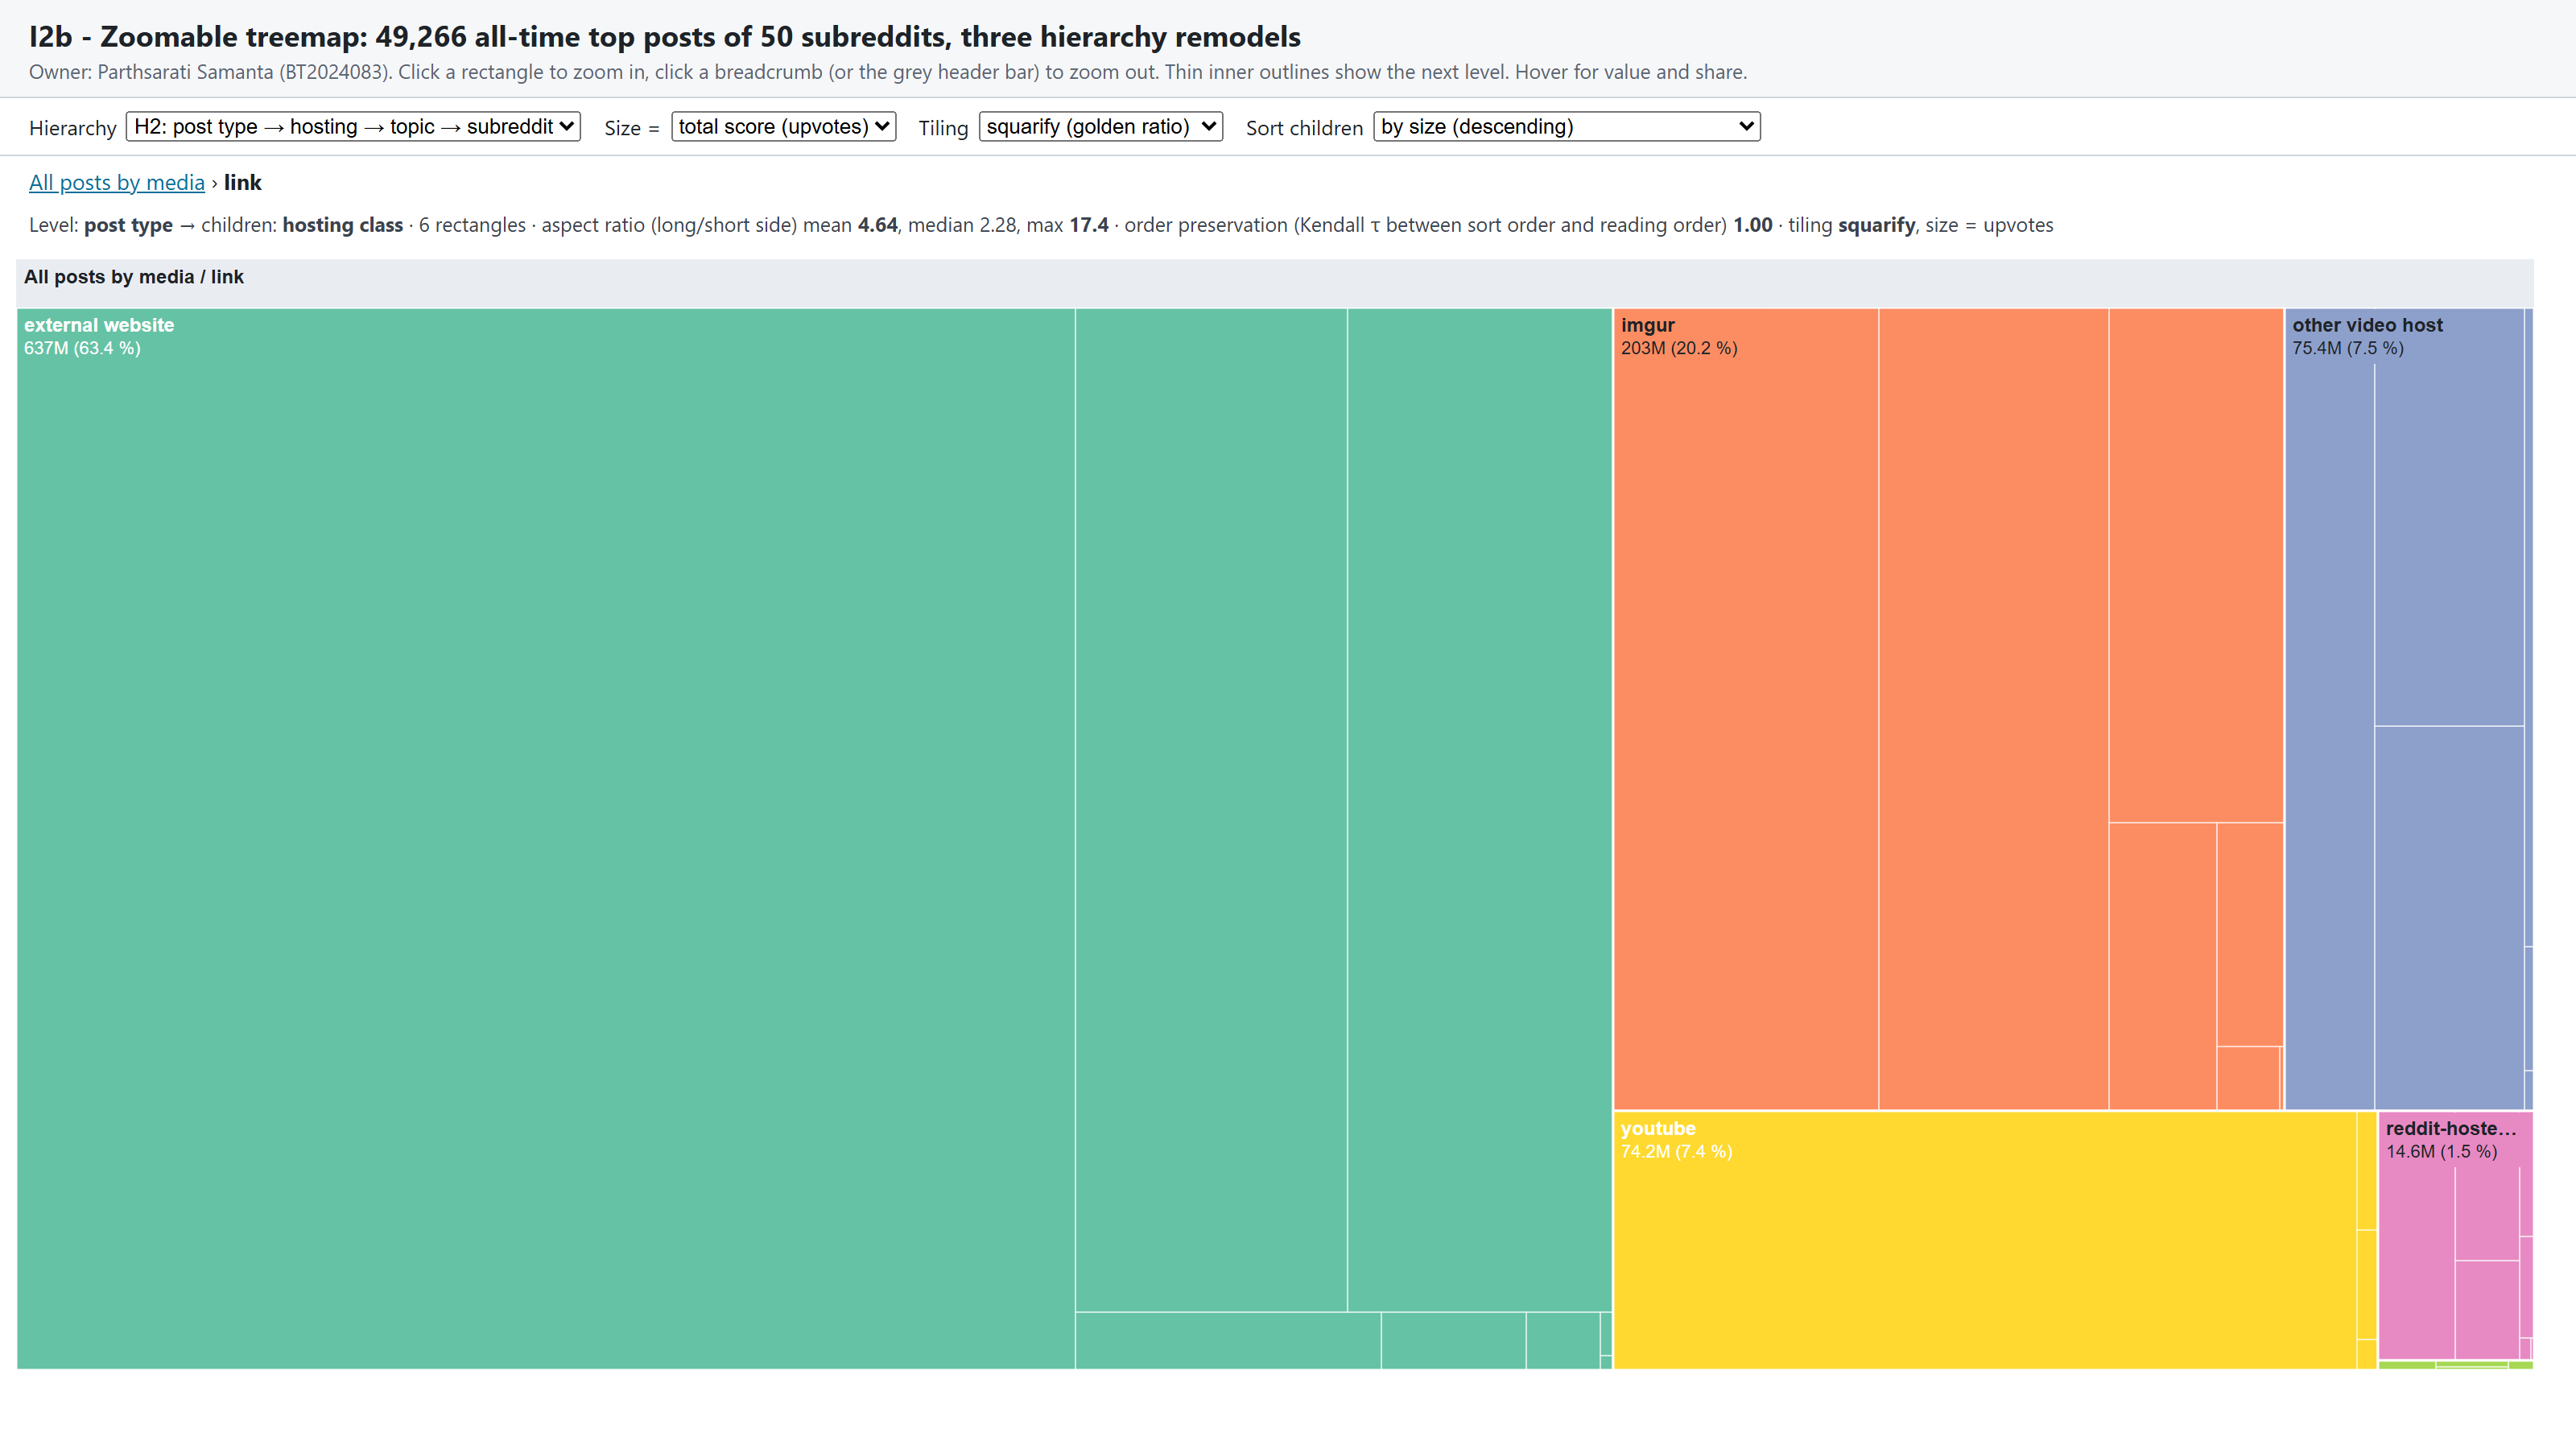
\includegraphics[width=0.495\textwidth]{Fig_33f_treemap_zoom_link_score.png}}
\caption{Zoomable treemap: three hierarchy remodels of the same 49,266 posts (a--c) and three zoom states (d--f), all with
squarify tiling. Files \fpath{Fig_33a..f_*.png}.}
\label{fig:33}
\end{figure*}

\textbf{Inferences (remodels and zoom, Fig.~\ref{fig:33}).}
(1) \textbf{H1 by posts} (Fig.~\ref{fig:33}a) is nearly uninformative at the subreddit level, because the dataset samples
about 1,000 posts per subreddit. Topic areas are proportional to how many subreddits each topic has, e.g.\
Entertainment 20.1\,\% with 10 subreddits. Zooming into Entertainment (Fig.~\ref{fig:33}d) confirms ten rectangles of
9.8--10.1\,\% each. The treemap thus exposes a \emph{sampling artefact}, and the measure must be changed before it can
answer a question about popularity.
(2) Switching the measure answers different questions. By \emph{total score}, Photos and curiosities lead with 22.6\,\%,
followed by News (18.8\,\%) and Memes (18.3\,\%), while Q\&A drops to 8.8\,\%. By \emph{total comments}, Q\&A leads with
29.6\,\% and News has 23.6\,\%, while Memes shrink to 6.0\,\%. Visual communities win upvotes and discussion communities
win comments, which repeats the A1 finding in a different visual form.
(3) \textbf{H2} (Fig.~\ref{fig:33}b) shows that links are the largest post type (41.0\,\%), followed by images (28.2\,\%),
text (26.6\,\%) and video (4.2\,\%). Zooming into links weighted by score (Fig.~\ref{fig:33}f) shows that external websites
take 63.4\,\% of link upvotes, imgur 20.2\,\%, other video hosts 7.5\,\% and YouTube 7.4\,\%. Text posts are always self
posts by definition, so H2's hosting level is degenerate for them, which is itself a validation of the classification.
(4) \textbf{H3} (Fig.~\ref{fig:33}c) shows the temporal skew of the corpus: 2019--20 holds 40.5\,\% of the posts, 2017--18
29.2\,\%, 2021--22 20.7\,\%, and the oldest and newest eras only 5.1\,\% and 4.5\,\%. Zooming to 2020 sized by comments
(Fig.~\ref{fig:33}e) shows that Q\&A alone produced 40.5\,\% of 2020's comments (10.4\,M), twice its post share. This is
consistent with heavy discussion during the 2020 lockdowns.
(5) Comparing remodels shows that the first level of the hierarchy decides what can be compared directly. Topics are
adjacent in H1, media types in H2 and time in H3. The same subreddit appears as one rectangle in H1 but is split
across four post types in H2 and across up to 14 years in H3.

\begin{figure*}[!t]
\centering
\subfloat[squarify]{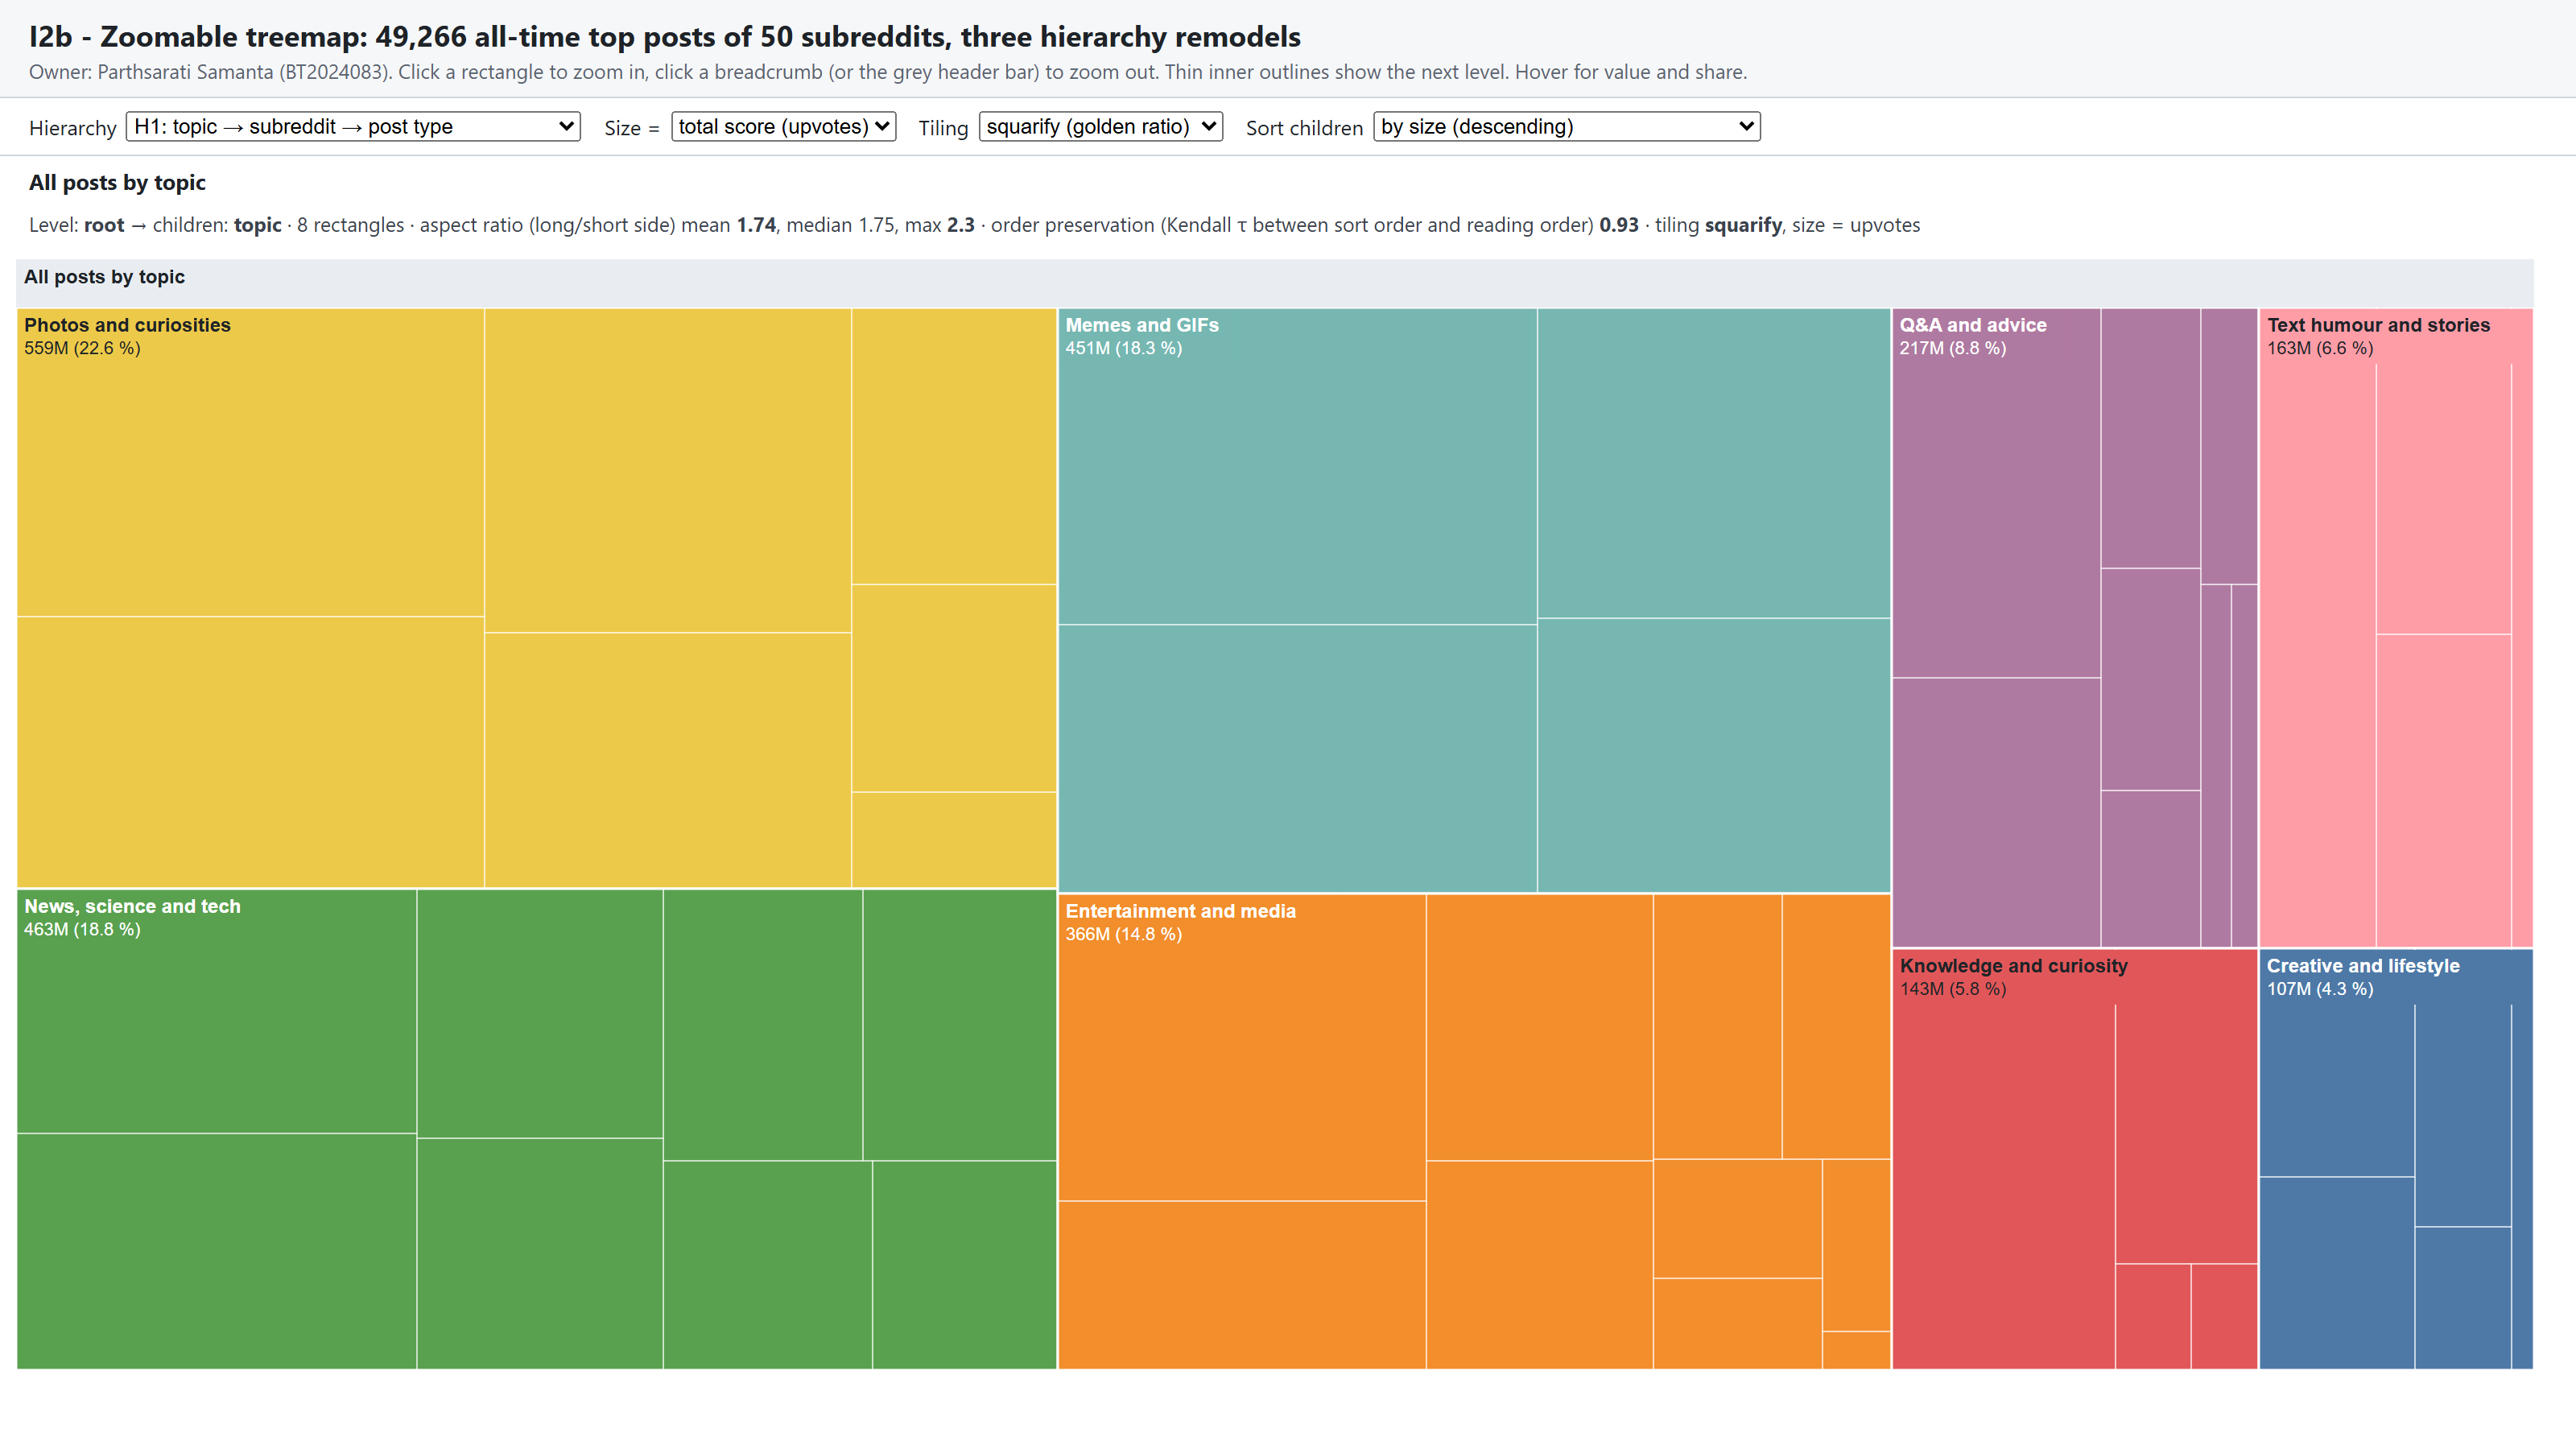
\includegraphics[width=0.33\textwidth]{Fig_34a_treemap_tiling_squarify.png}}\hfill
\subfloat[binary]{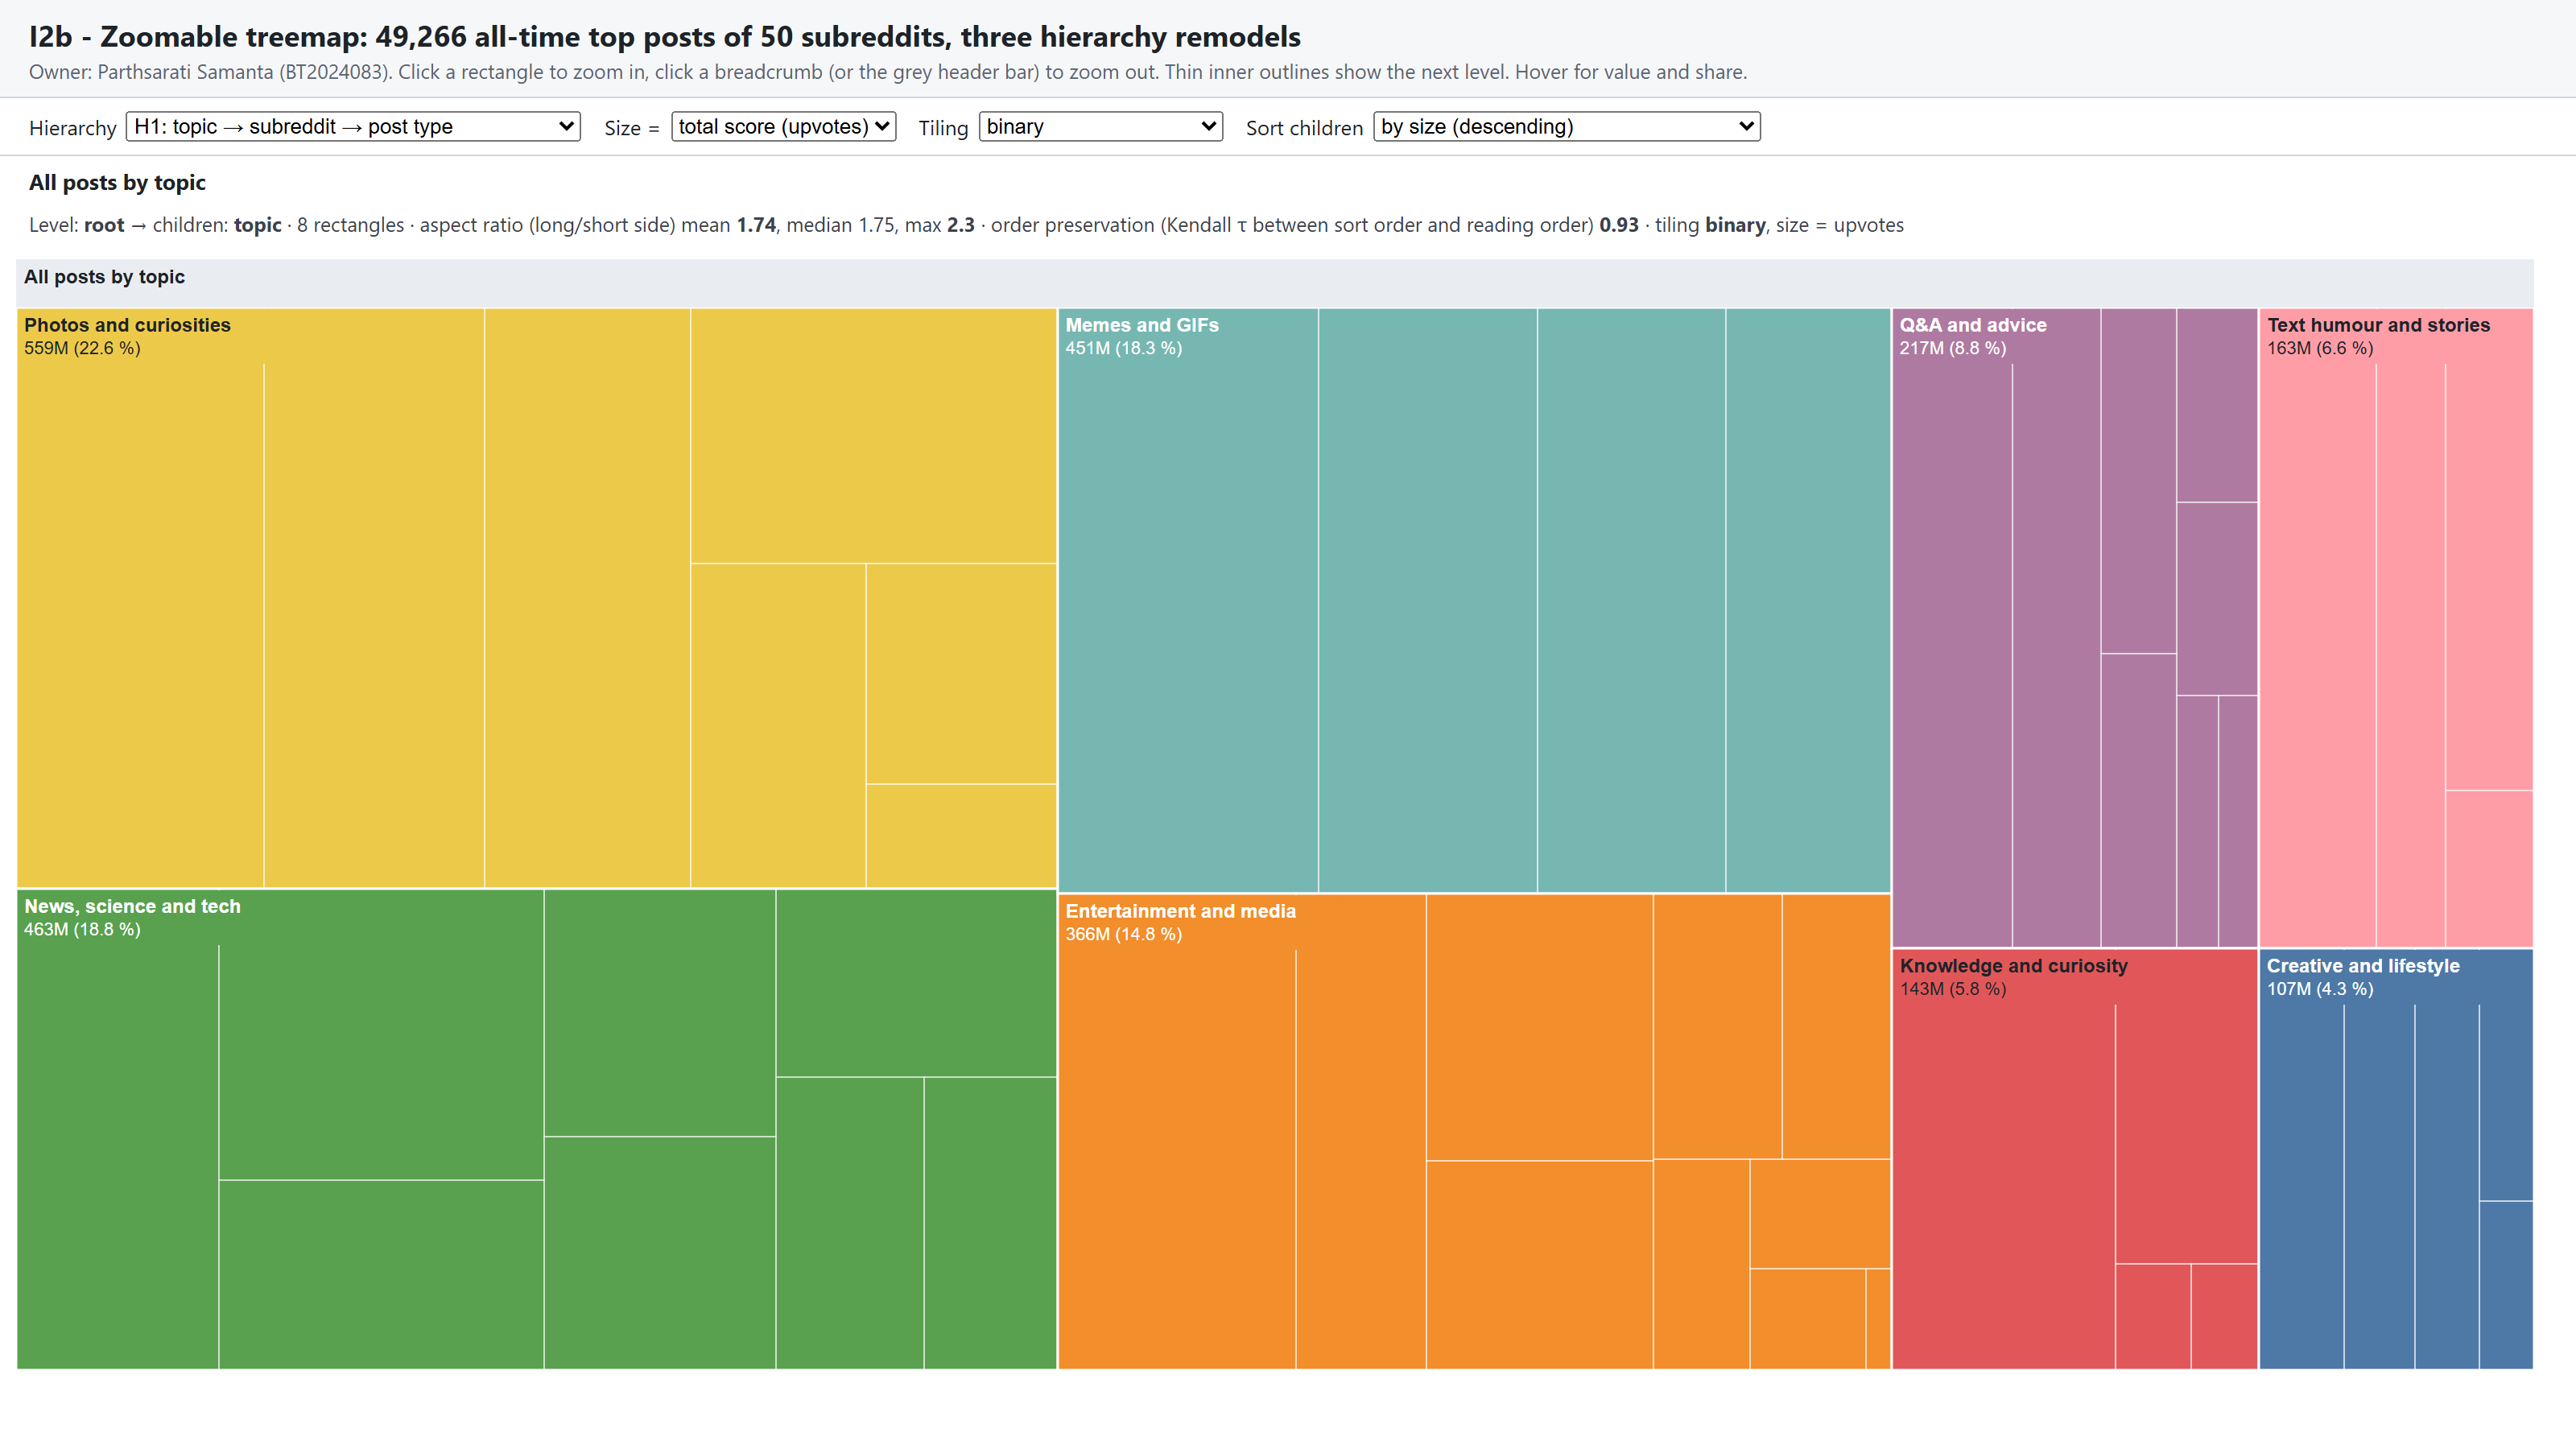
\includegraphics[width=0.33\textwidth]{Fig_34b_treemap_tiling_binary.png}}\hfill
\subfloat[slice]{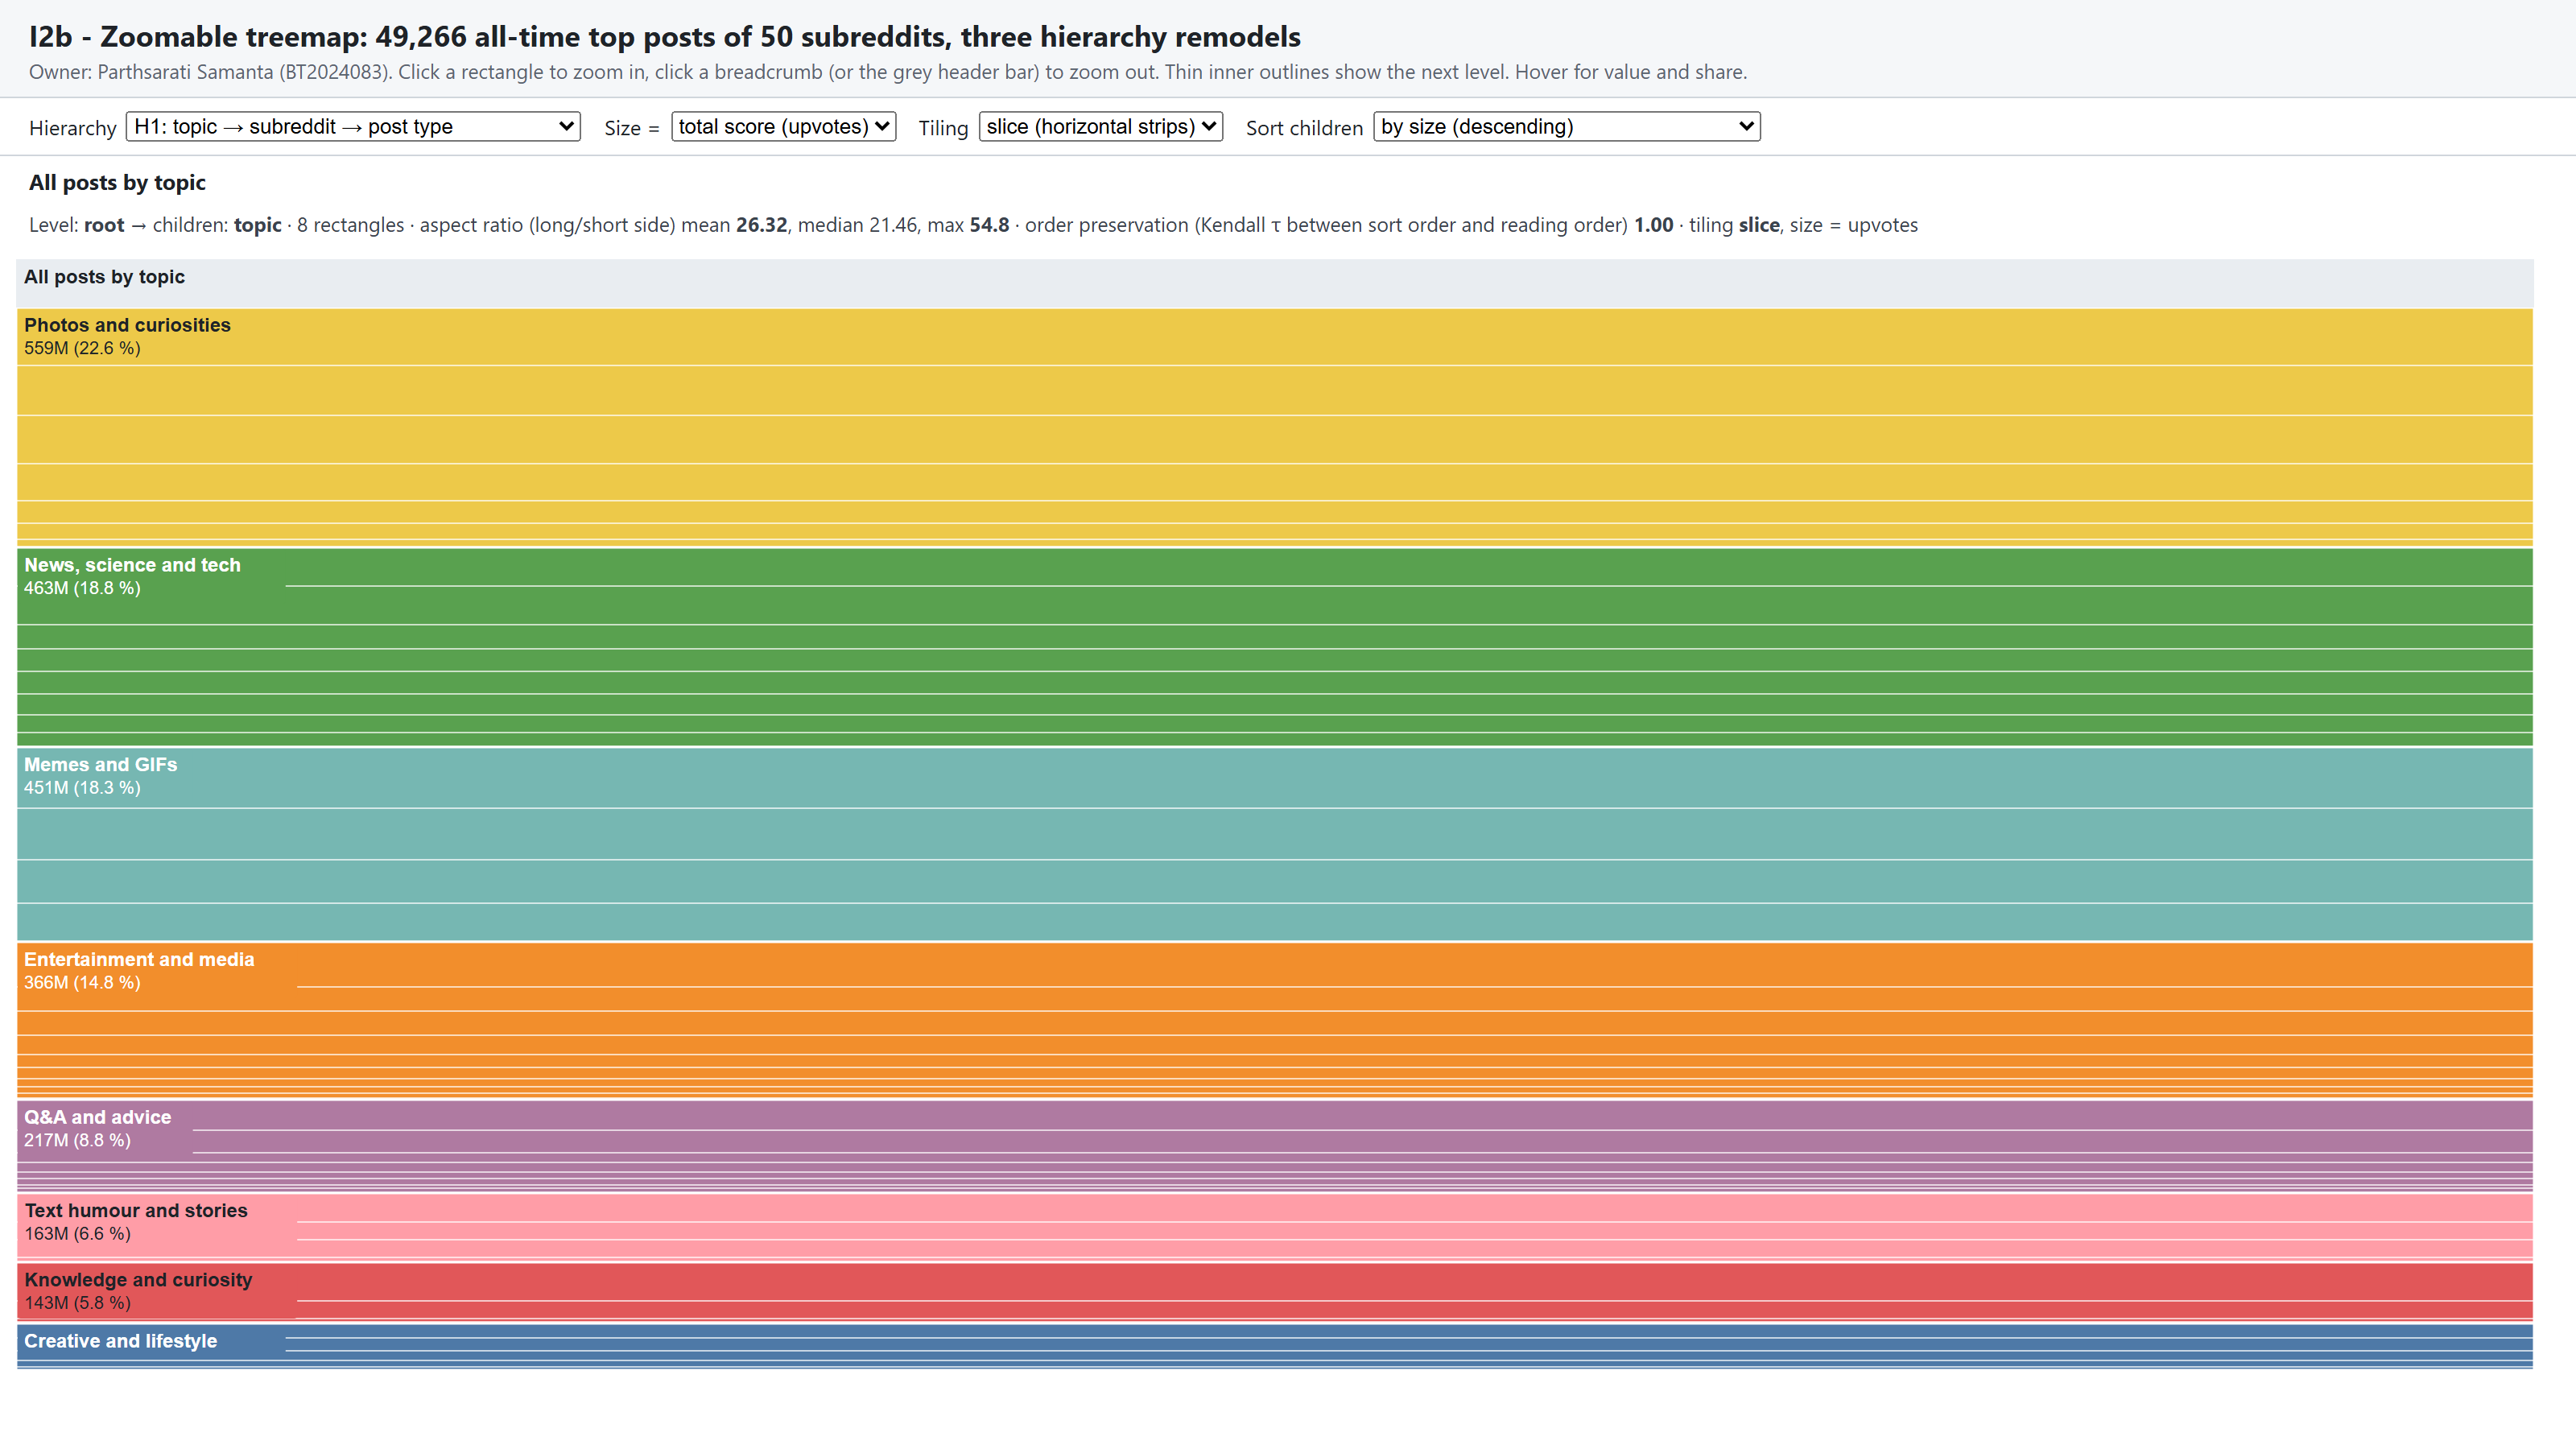
\includegraphics[width=0.33\textwidth]{Fig_34c_treemap_tiling_slice.png}}\\
\subfloat[dice]{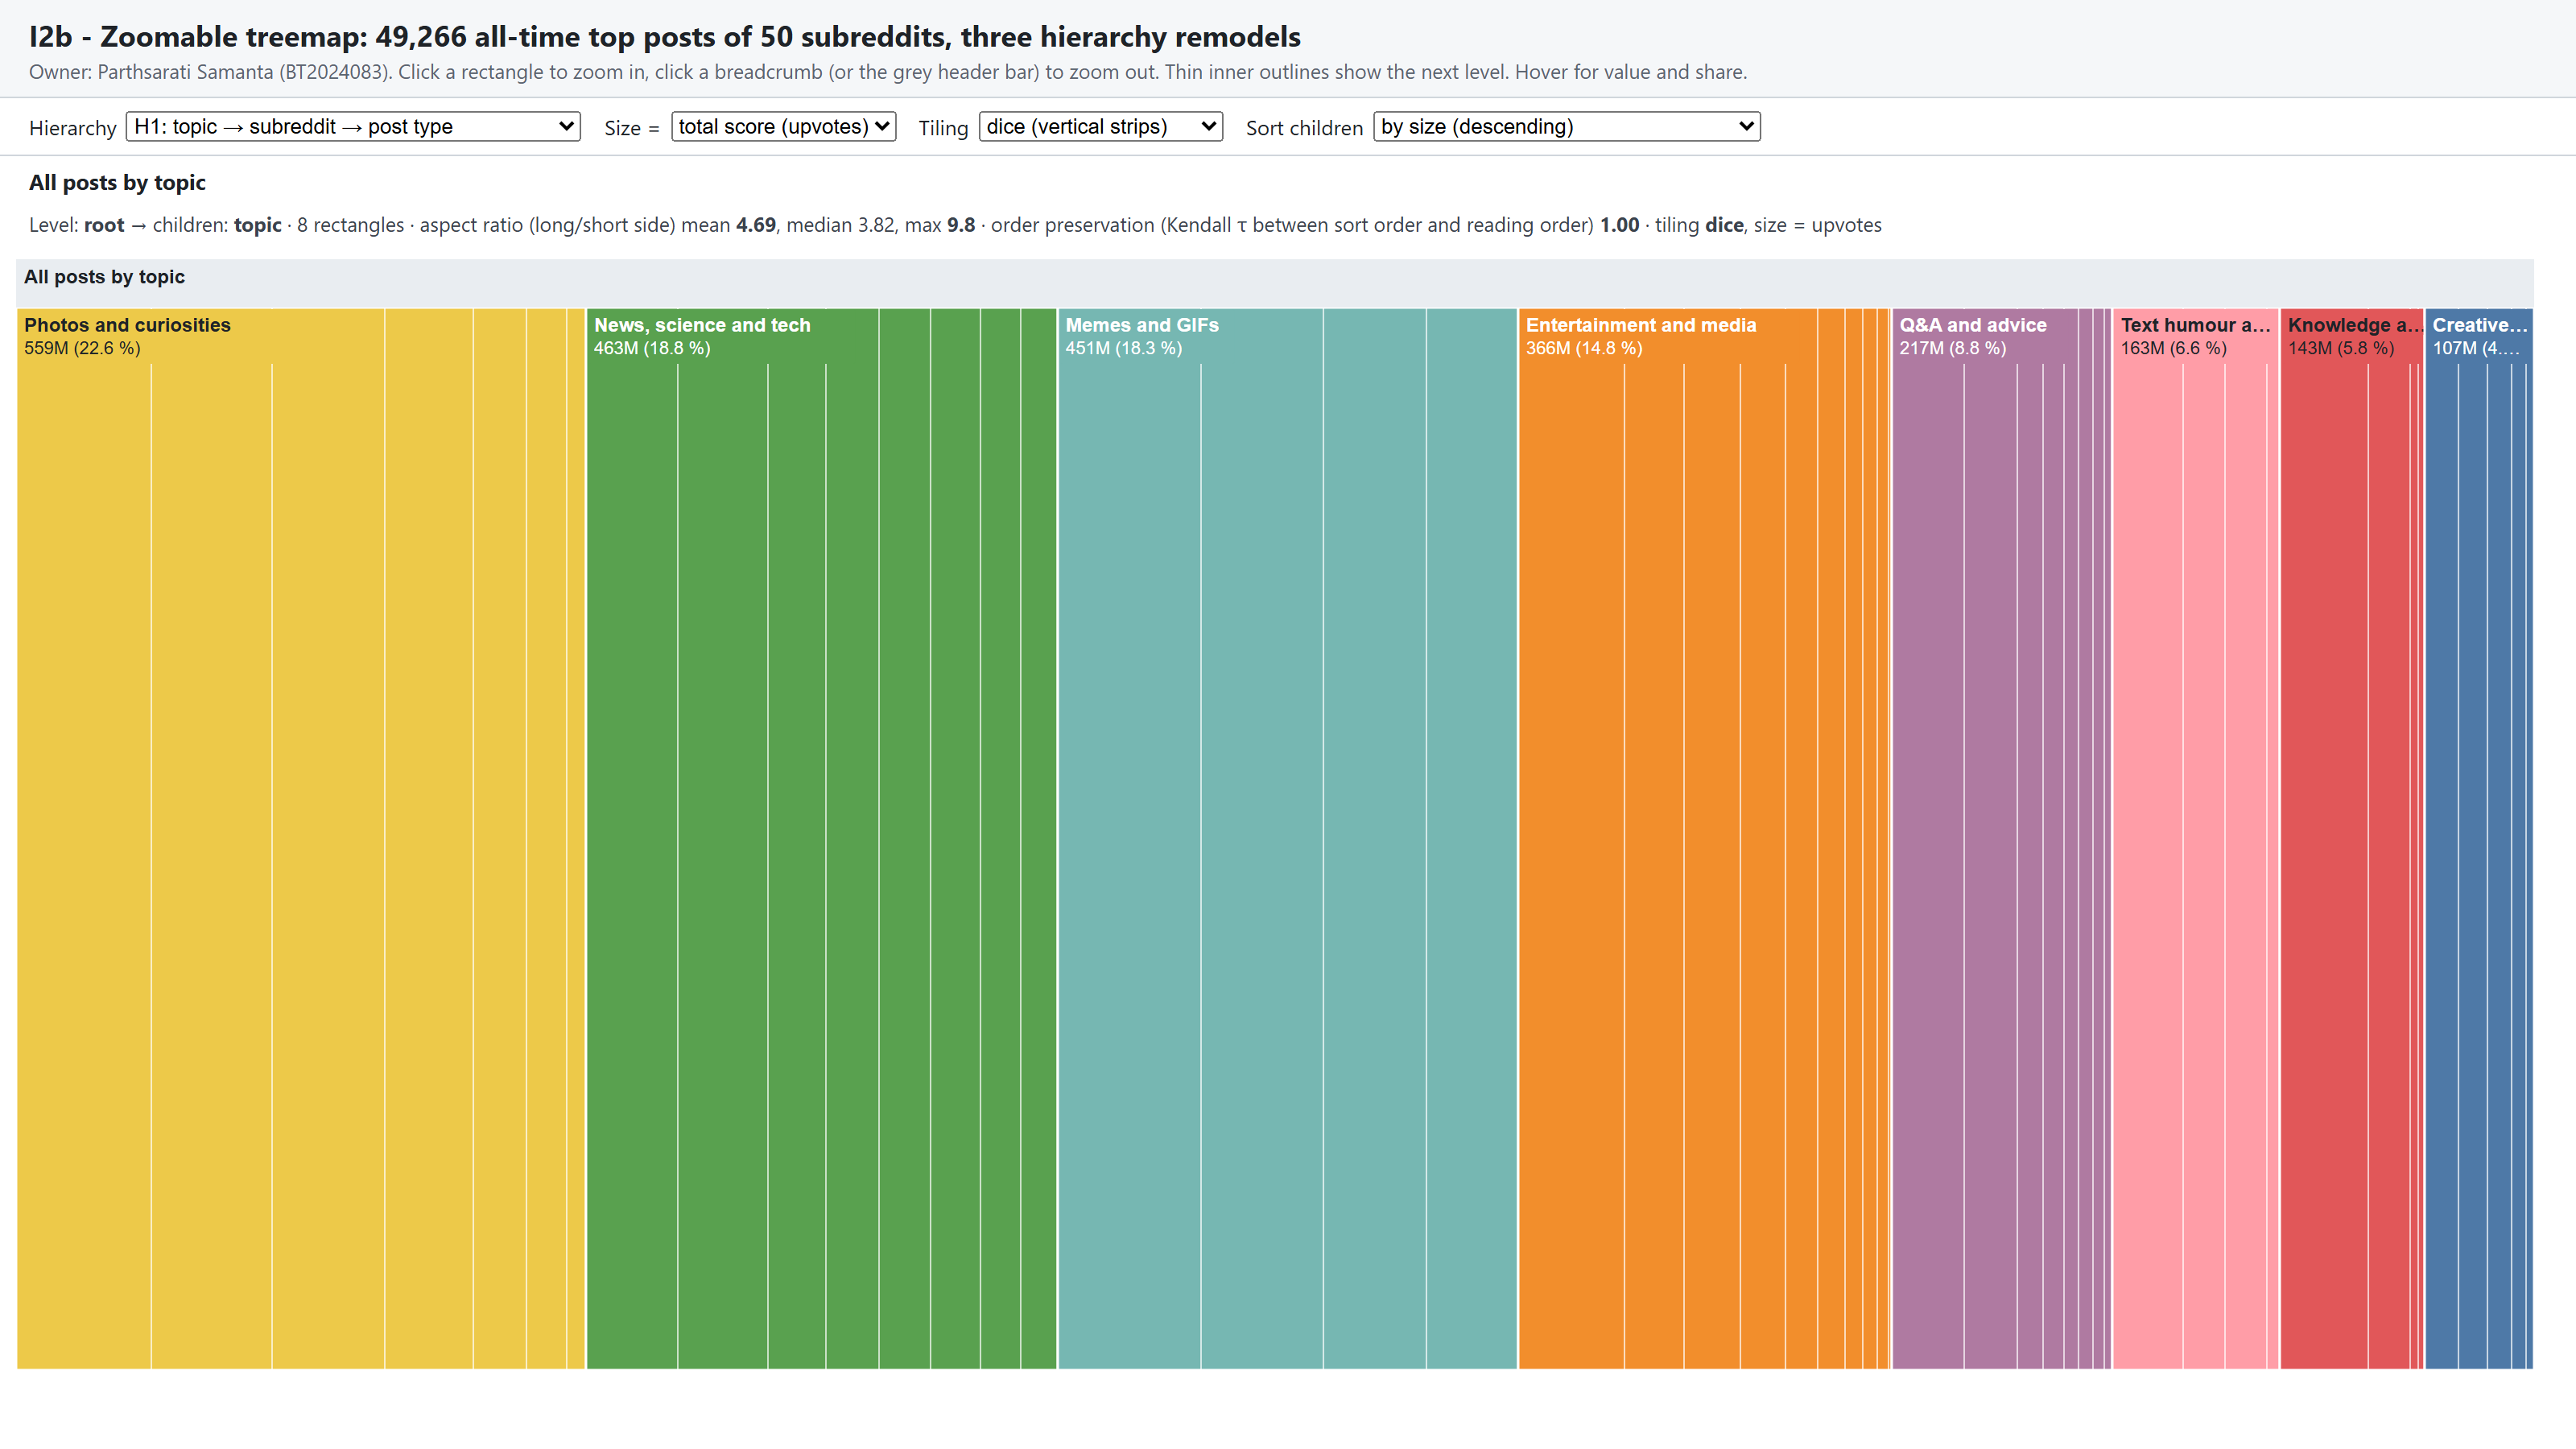
\includegraphics[width=0.33\textwidth]{Fig_34d_treemap_tiling_dice.png}}\hspace{0.02\textwidth}
\subfloat[slice-dice]{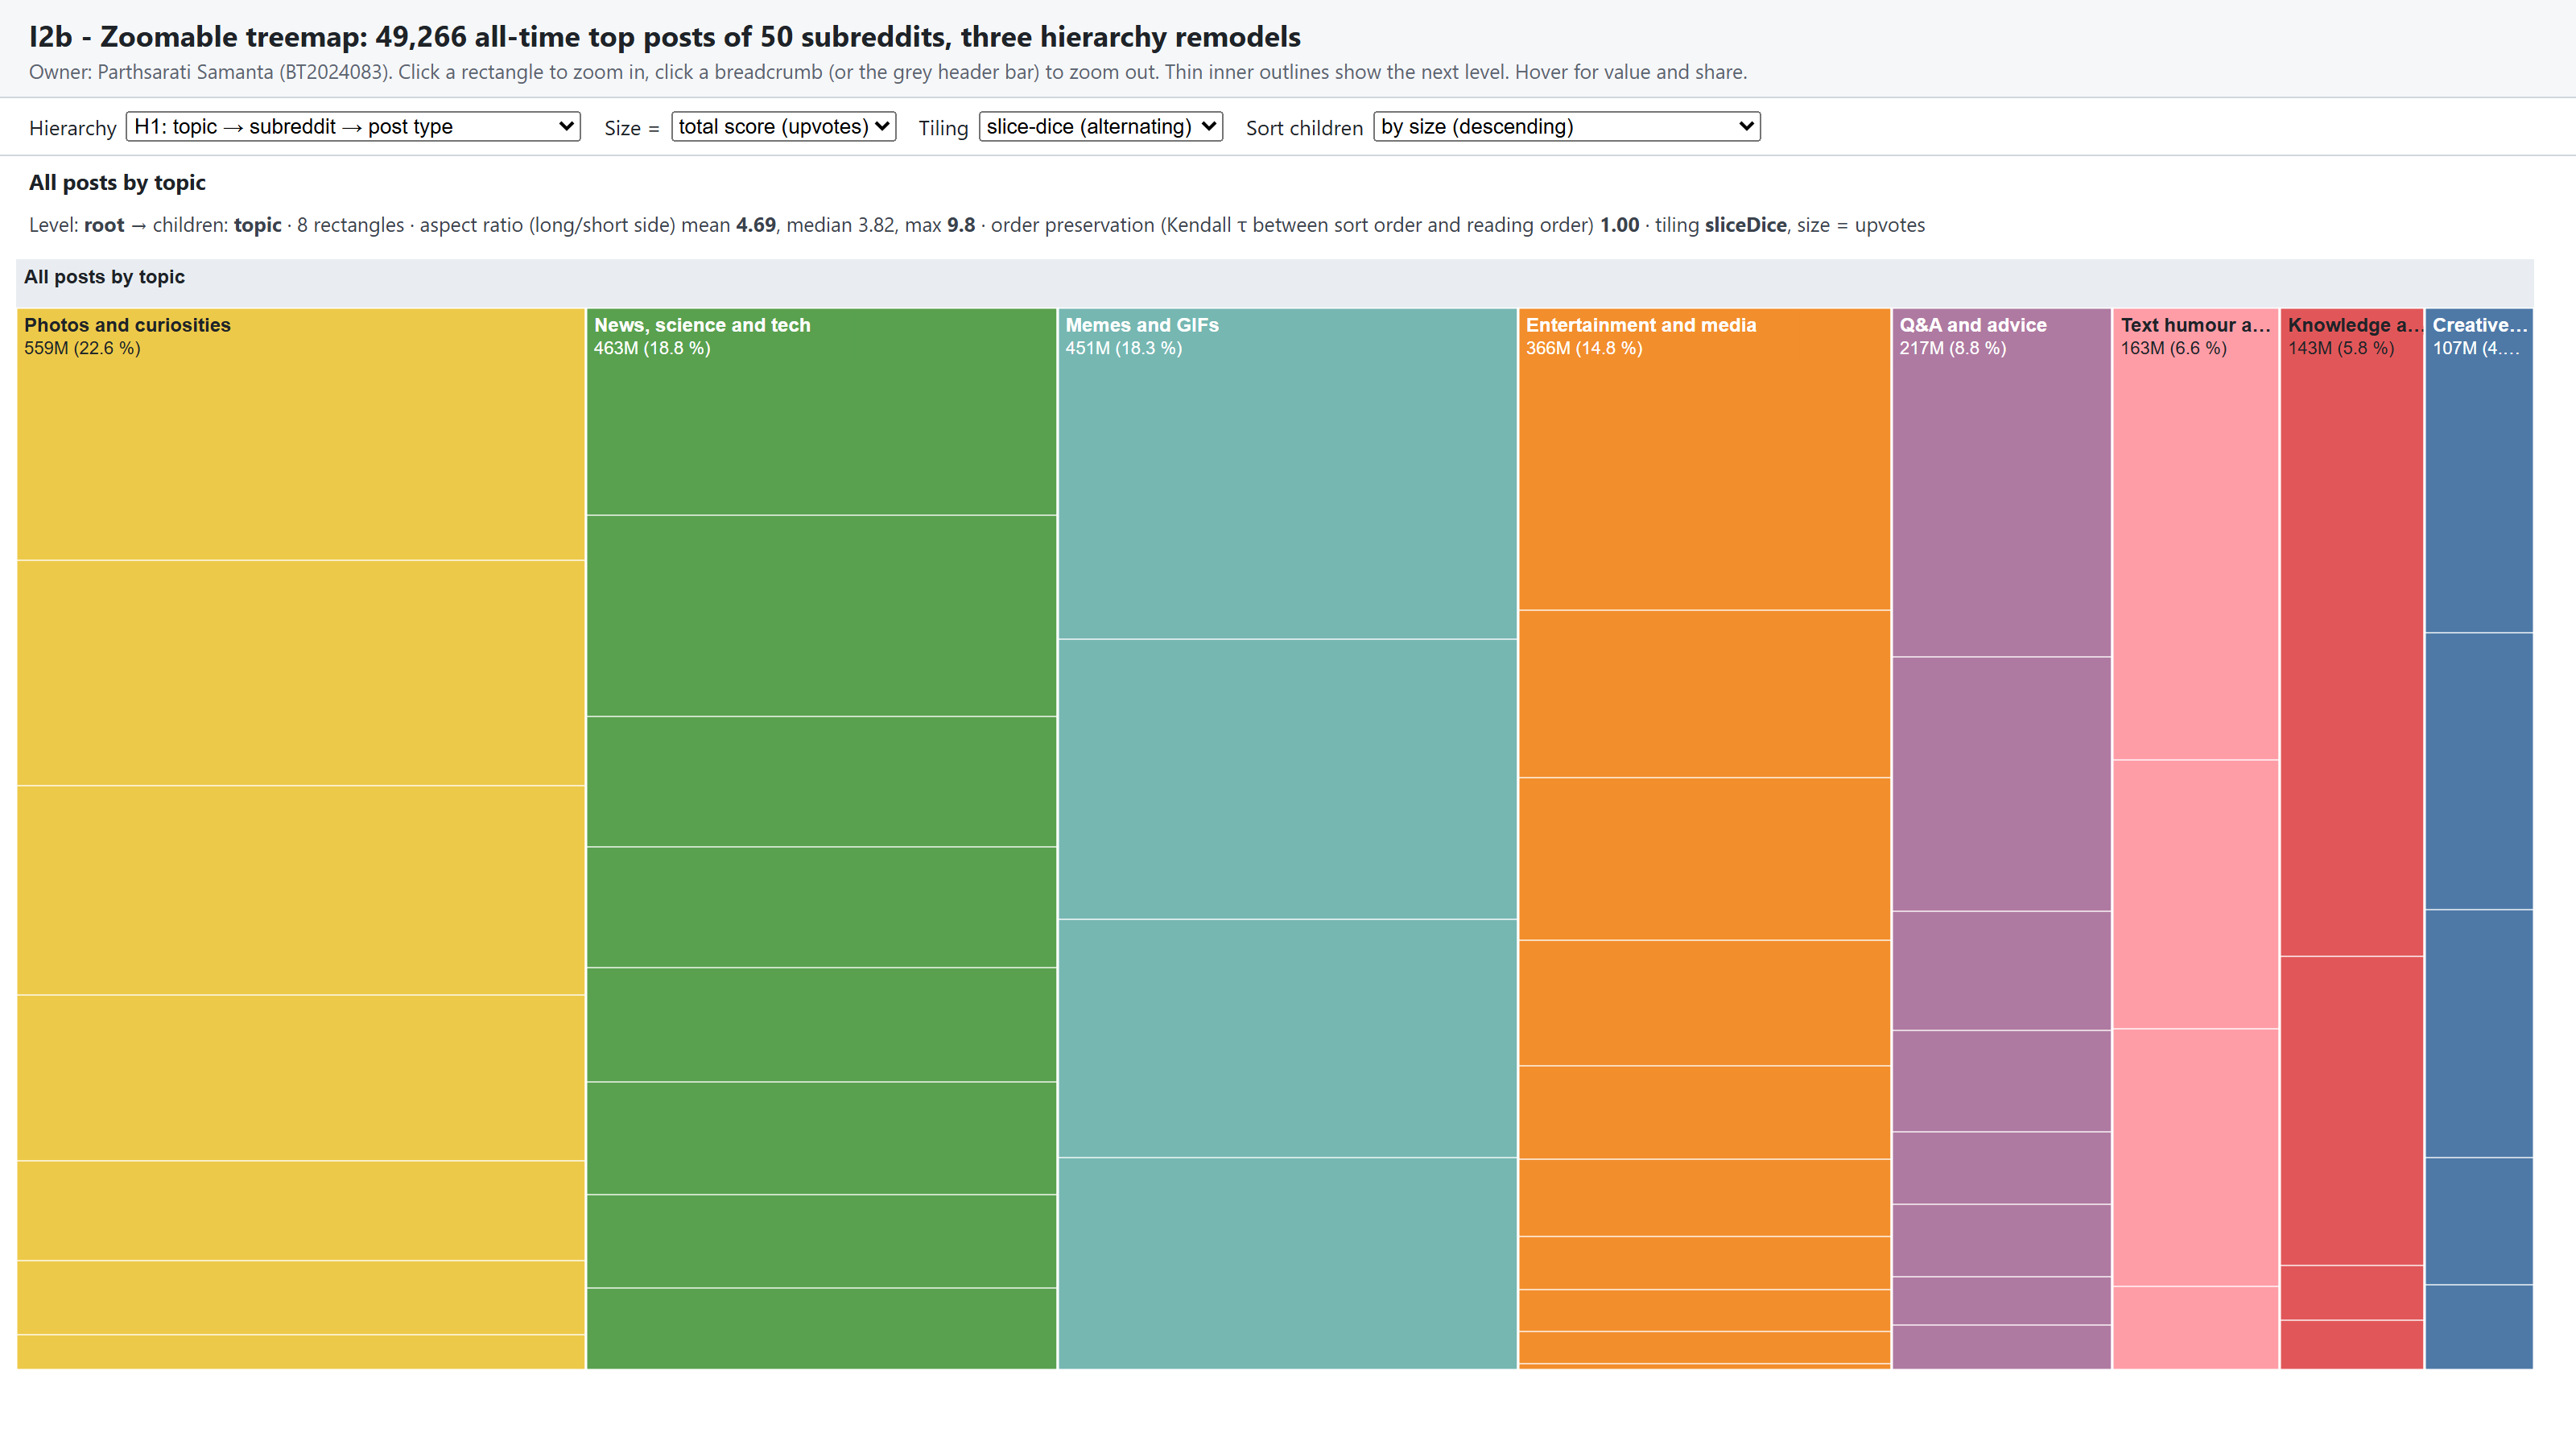
\includegraphics[width=0.33\textwidth]{Fig_34e_treemap_tiling_sliceDice.png}}
\caption{The five tiling strategies on the same view (H1 root, size = total score, children sorted by size). Files
\fpath{Fig_34a..e_*.png}.}
\label{fig:34}
\end{figure*}
\input{generated/tab_tiling}

\textbf{Inferences (tiling, Fig.~\ref{fig:34}, Table~\ref{tab:tiling}).}
(1) Squarify and binary give near-square rectangles (mean aspect ratio 1.6--2.2), which makes areas easy to compare and
leaves room for labels. Their worst cases (5.4--10.0) all occur in the H2 root, where the video category holds only
4\,\% of posts and must become a strip. Binary is the most balanced overall (mean 1.56 when sorted by size).
(2) Slice and dice keep the sort order perfectly ($\tau=1$) but produce extreme slivers: slice has a mean aspect ratio of
18.9 and a worst case of 56.3. In Fig.~\ref{fig:34}c the eight topics
become thin full-width strips. That is fine for ordered categories such as eras or years, but small items such as
Creative and lifestyle cannot be labelled.
(3) Slice-dice alternates direction by depth. It is good at the root (mean 3.8) but inherits slice's slivers one level
down (23.7 in the Entertainment view), and it preserves order.
(4) Squarify is the only tiling whose order preservation is below 1 ($\tau$ = 0.95--0.97). Its greedy rows place items out
of reading order, so ``what is next to what'' carries no meaning. Binary keeps $\tau\approx1$ with good aspect ratios.
For the chronological H3 hierarchy sorted by name, binary or slice-dice are therefore preferable, while squarify is best
for comparing magnitudes.

\subsection{Observations and limitations (I2)}
Bundling makes cluster structure readable in a 2,000-line plot, brushing turns it into a query tool, and reordering exposes
pairwise relations; the bundled view should be confirmed in the unbundled one. The treemap's value depends on choosing the
hierarchy and the measure deliberately; it also revealed the per-subreddit sampling design. Limitations: the
parallel-coordinates sample is 4\,\% of the corpus, and SVG rendering becomes sluggish beyond about 5,000 lines (canvas
would be needed). Treemaps cannot show negative or non-additive measures such as medians.
